\documentclass[11pt]{article}
\usepackage{graphicx} % Required for inserting images
\usepackage{amsmath}
\usepackage{lipsum}
\usepackage{pdfcomment}

\usepackage[table,xcdraw]{xcolor} % Enable table colors and HTML color codes
\usepackage{subcaption}
\usepackage{hyperref} % Include the hyperref package
\usepackage[english]{babel}
\usepackage[utf8]{inputenc}
\usepackage{amsfonts}
\usepackage{longtable}
\usepackage{booktabs}
\usepackage{float} 
\usepackage{geometry}
\usepackage{lineno}
\usepackage{authblk}
\usepackage{tcolorbox}
\usepackage{cite}

%font type and line spacing
% \usepackage{mathpazo}
% \usepackage{mathptmx}
\usepackage{lmodern} 
\renewcommand{\baselinestretch}{1.5}


\usepackage{array}
\usepackage{multirow}

\usepackage{amssymb}
\usepackage{pifont}


\usepackage[colorinlistoftodos]{todonotes}

% \usepackage{times}

%chinese
% \usepackage{xeCJK}

\usepackage{wrapfig}

%remove all paragraph indent
% \usepackage{parskip}

% Use BibTeX for bibliography management (uncomment this if author name is needed.
% \usepackage[semicolon]{natbib}
\usepackage[numbers,sort]{natbib}
\usepackage{cite}

%margin
\geometry{
    left=1in,
    right=1in,
    top=1in,
    bottom=1in
}

\hypersetup{
    colorlinks=true, % Enable colored links
    linkcolor=blue,  % Set the color of internal links (e.g., references)
    citecolor=blue, % Change this color as desired
    urlcolor=blue    % Set the color of external links (e.g., URLs)
}

\usepackage{amsthm}
\newtheorem{example}{Example}[section] % Define the example environment
\newtheorem{homework}{Homework} % Define the example environment


\usepackage{titlesec}
\usepackage{titletoc}
% Define \subsubsubsection
\titleclass{\subsubsubsection}{straight}[\subsection]
\newcounter{subsubsubsection}[subsubsection]
\renewcommand\thesubsubsubsection{\thesubsubsection.\arabic{subsubsubsection}}
\titleformat{\subsubsubsection}{\normalfont\normalsize\bfseries}{\thesubsubsubsection}{1em}{}
\titlespacing*{\subsubsubsection}{0pt}{3.25ex plus 1ex minus .2ex}{1.5ex plus .2ex}
\setcounter{secnumdepth}{4} % Numbering depth
\setcounter{tocdepth}{4} % Include subsubsubsections in the table of contents

% % Set section headings to 10pt
\titleformat*{\section}{\fontsize{11}{12}\selectfont\bfseries}
\titleformat*{\subsection}{\fontsize{11}{12}\selectfont\bfseries}
\titleformat*{\subsubsection}{\fontsize{11}{12}\selectfont\bfseries}
\titleformat*{\paragraph}{\fontsize{11}{12}\selectfont\bfseries}
\titleformat*{\subparagraph}{\fontsize{11}{12}\selectfont\bfseries}

% Adjust the formatting in the table of contents
\titlecontents{subsubsubsection}
[8em] % adjust this value to fit your needs
{\small}
{\hyperlink{toc.\thecontentslabel}{\thecontentslabel.} }
{}
{\ \titlerule*[.5pc]{.}\contentspage}

\titlespacing*{\subsubsubsection}{0pt}{3.25ex plus 1ex minus .2ex}{1.5ex plus .2ex}

\usepackage{caption}
% Make the label bold and keep the caption text regular
\captionsetup{
  labelfont=bf, % makes label (e.g., "Figure 1") bold
  textfont=normal % keeps caption text in normal font
}


% \usepackage{sectsty}
% % Remove indentation after section headings
% \sectionfont{\noindent}

%remove hyphenation
\usepackage{microtype}


\usepackage{enumitem}
% Set item separation globally
\setlist{itemsep=0em}

% % Adjust the space after figure captions
% \setlength{\belowcaptionskip}{-15pt}

\usepackage{fancyhdr} % For custom headers/footers
\usepackage{lastpage} % For total number of pages

\pagestyle{fancy}
\fancyhf{} % Clear header/footer
% \fancyfoot[C]{\thepage\ of \pageref{LastPage}} % Page number as x out of total
\renewcommand{\headrulewidth}{0pt} % Remove horizontal line from header


\usepackage{listings}
\usepackage{xcolor}


\definecolor{codegreen}{rgb}{0,0.6,0}
\definecolor{codegray}{rgb}{0.5,0.5,0.5}
\definecolor{codepurple}{rgb}{0.58,0,0.82}
\definecolor{backcolour}{rgb}{0.95,0.95,0.92}

\lstdefinestyle{mystyle}{
    backgroundcolor=\color{backcolour},   
    commentstyle=\color{codegreen},
    keywordstyle=\color{magenta},
    numberstyle=\tiny\color{codegray},
    stringstyle=\color{codepurple},
    basicstyle=\ttfamily\footnotesize,
    breakatwhitespace=false,         
    breaklines=true,                 
    captionpos=b,                    
    keepspaces=true,                 
    numbers=left,                    
    numbersep=5pt,                  
    showspaces=false,                
    showstringspaces=false,
    showtabs=false,                  
    tabsize=2
}

\lstset{style=mystyle}

\begin{document}
% \newgeometry{top=1in, bottom=1in, left=1.5in, right=1.5in}
% \maketitle

\title{Walkability Assessment Using Multimodal Learning from Street View Images}

\author[1]{\normalsize Prathyush Kumar Reddy Lebaku}
\author[1]{Lu Gao, Ph.D. \thanks{lgao5@central.uh.edu}}
\author[2]{Kailai Wang, Ph.D.}
% \author[1]{xxxx}
\author[3]{Jingran Sun, Ph.D.}

\affil[1]{Department of Civil and Environmental Engineering, University of Houston}
\affil[2]{Department of Industrial Engineering, University of Houston}
\affil[3]{Department of Civil and Environmental Engineering, University of South Florida}


\date{}

\maketitle       

% Enable line numbering
\linenumbers 


\newpage
\section*{Abstract}
Walkability reflects how supportive an environment is for walking, social interaction, and community well-being. Accurate and scalable assessment of walkability is crucial for urban planning, asset management, and improving pedestrian infrastructure. This study presents a multimodal learning framework for evaluating street-level walkability using image-based data. We first implement transfer learning with several pre-trained image classification models, followed by ensemble learning to boost performance. The ensemble model achieves an accuracy close to 90\% in classifying pedestrian environments into three walkability levels. Beyond vision-only models, we incorporate Vision-Language Models (VLMs) to generate detailed textual descriptions of street scenes. These descriptions are then classified using a fine-tuned BERT model, which yields up to 85.4\% accuracy. We also explore direct classification using VLMs without an intermediate classifier, though this approach performs less reliably. Our results demonstrate that both image-based and multimodal pipelines are effective for walkability assessment, with ensemble CNNs and VLM-BERT combinations offering the most robust performance. The proposed framework supports large-scale, automated evaluation of pedestrian environments, aiding future planning and decision-making for safer and more walkable cities.


\textbf{Keywords:} Walkability Assessment, Multimodal Learning, Vision-Language Models, Street View Imagery, Urban Planning 

\section{Introduction}
Pedestrian friendliness pertains to the extent to which an area encourages and supports activities such as walking, biking, and social interactions. Studies have demonstrated that the presence of walkable streets and urban spaces positively impacts the social and economic well-being of communities \citep{ma2023quantitative}. It is important for planners and other professionals to be aware of the condition of their community’s walking environment and make appropriate asset management and resource allocation decisions. Gaining a comprehensive understanding of how the physical design and visual elements of the built environment influence the pedestrian experience is crucial for developing strategies that enhance the pedestrian-friendliness of neighborhoods. 

% Recent research has witnessed new developments in the adoption of cutting-edge deep learning techniques to evaluate the walkability of urban neighborhoods. Using various image sources such as Google Street View and self-collected images, researchers have identified important elements like pedestrian count, sky portion, trees, obstacles, pavement, and buildings. Subject opinions were collected to understand perceptions related to walkability, including security, depression, vitality, and aesthetics. These studies have utilized semantic segmentation, image classification, object detection, and other methodologies to analyze the urban environment and predict walkability scores based on the presence and composition of different objects. For instance, \citet{yin2015big} explored the extraction of pedestrian count data using machine vision and learning technology from Google Street View images. In another study, \citet{yin2016measuring} developed a method based on semantic segmentation from Google Street View imagery to identify sky areas, enabling the calculation of sky proportions and revealing correlations between visual enclosure measures, pedestrian volume, and walk score. \citet{zhou2019social} employed a semantic segmentation approach to extract valuable information such as trees, obstacles, sky, pavement, road, and buildings from Baidu street images. They used this information to compute indicators like psychological greenery, visual crowdedness, outdoor enclosure, and visual pavement, which were combined into a composite index called integrated visual walkability. Their comparison with manual interpretation yielded an accuracy of 78.5\%. \citet{nagata2020objective} developed a deep learning method utilizing semantic segmentation on Google Street View pictures to evaluate walkability. Similarly, \citet{wei2022mapping} employed a deep learning-based image classification approach using street view images to map human perceptions at the parcel level in Shanghai. Results showed that highly urbanized areas were perceived as more secure and vital but also more depressing, especially in the Puxi district within the Inner Ring Road. \citet{doiron2022predicting} utilized semantic segmentation and object detection methods to extract valuable information, such as persons, bicycles, buildings, sidewalks, sky, and vegetation, from Google Street View images. In a different study, \citet{han2022measuring} employed semantic segmentation techniques to explore the connection between the urban built environment and the psychological stress experienced by residents in Seoul’s Gangnam District. By classifying visual elements in street views and correlating the results with stress perception ratings, they gained insights into this relationship. \citet{li2022measuring} proposed a virtual reality panoramic image-based deep learning framework to measure visual walkability perception and identify the visual features that make urban streets attractive for walking. Their deep learning-based image classification model achieved over 90\% accuracy in predicting street views in six categories related to walkability perception: walkability, feasibility, comfort, pleasurability, accessibility, and safety. They then used a regression model to assess the correlation between different objects and the six perception categories based on semantic segmentation. Lastly, \citet{kang2023assessment} developed a semantic segmentation-based method to assess walkability in Jeonju City, Korea, considering both physical and perceived aspects. They trained a deep learning model on street view images to accurately predict perceived walkability. 


Recent work has evolved from counting isolated features to modeling street scenes, which links physical elements to perceived walkability. Researchers utilize street-view imagery and VR panoramas to analyze visual composition. They apply semantic segmentation, object detection, and classification to quantify elements such as sky openness, vegetation, sidewalks, buildings, and the presence of pedestrians or bicycles. These analyses are then correlated with perceptions like security, vitality, aesthetics, comfort, accessibility, feasibility, safety, and stress. Early efforts operationalized concrete proxies (e.g., pedestrian counts; sky fraction as visual enclosure) and showed associations with pedestrian volume and walk score \citep{ki2023novel}. Subsequent work integrated multi-element segmentation to build composite indices (e.g., integrated visual walkability, percentage of agreement with manual interpretation) and to generalize across platforms and cities \citep{wang2024investigating}. More recent studies map human perceptions at parcel or neighborhood scales and uncover spatial heterogeneity and connect built-form composition to stress ratings \citep{lei2024evaluating}. 

% Methodological advances also include immersive data sources and two-stage pipelines that pair high-accuracy perception classification with regressions on segmented objects to interpret what drives perceived walkability \citep{li2022measuring}. City-scale assessments that jointly consider physical and perceived factors further show that trained segmentation models can predict perceived walkability with high fidelity \citep{kang2023assessment}.

% These studies on neighborhood walkability highlights the importance of accurately understanding and improving pedestrian experiences in urban environments. However, fully automating walkability measurement and capturing subjective pedestrian perceptions remain challenging, especially when relying solely on basic image classification. To address these gaps, this study goes beyond traditional image classification by integrating multiple approaches, including transfer learning, ensemble modeling, and vision-language pipelines with BERT. Through comparative experiments on a labeled street-view dataset, we assess how each method handles the complexity of street environments and whether combining visual and textual cues leads to more accurate and robust walkability predictions.

Recent studies on walkability have shown progress in using vision-based methods to analyze street images and identify elements such as sidewalks, trees, and buildings. These approaches are effective for capturing objective features of the built environment, but they still face challenges in reflecting subjective pedestrian perceptions, especially when relying only on basic image classification. To address this limitation, our study introduces an approach that combines transfer learning, CNN ensemble modeling, and a vision-language pipeline where a VLM generates scene descriptions and a BERT classifier interprets them. Using a labeled street-view dataset, we compare these methods to examine their performance in complex street settings and assess whether integrating visual and textual cues can produce more accurate, robust, and interpretable walkability predictions.

\section{Literature Review}

\subsection{Traditional Approaches to Walkability Assessment}

Traditional methods predominantly rely on environmental audits, which involves on-site evaluations of pedestrian infrastructure and urban design features. While these audits provide granular insights into walkability factors like sidewalk quality or street connectivity, they are labor-intensive, costly, and challenging to scale across large urban areas. Subjective evaluations, such as surveys or expert assessments, further compound these issues due to inconsistencies in perceptual judgments and a lack of standardized metrics. For instance, field surveys evaluating visual enclosure (a key determinant of pedestrian comfort) are prone to inter-rater variability, which undermines their reliability for comparative analyses \citep{dai2024street}.

To mitigate scalability constraints, computer-aided audits leveraging tools like Google Street View (GSV) emerged as alternatives to in-person evaluations \citep{koo2022a}. However, manual virtual audits remain time-consuming and fail to systematically capture the dynamic perceptual experiences of pedestrians, such as real-time visual or spatial interactions. Traditional frameworks also emphasize macroscale factors, including employment density, land use diversity, and intersection density. While these metrics provide broad insights into neighborhood walkability, they overlook streetscape features, such as building proportions, greenery, or sidewalk aesthetics, which critically influence pedestrian behavior and comfort \citep{koo2022b}.

\subsection{Vision-Based Methods}


Recent research has witnessed developments in the adoption of vision-based techniques to evaluate the walkability of urban neighborhoods, as outlined in Table \ref{tab:papers}. Using various image sources such as Google Street View and self-collected images, researchers have identified important elements like pedestrian count, sky portion, trees, obstacles, pavement, and buildings. Subject opinions were collected to understand perceptions related to walkability, including security, depression, vitality, and aesthetics. These studies have utilized semantic segmentation, image classification, object detection, and other methodologies to analyze the urban environment and predict walkability scores based on the presence and composition of different objects. For instance, \citet{yin2015big} explored the extraction of pedestrian count data using machine vision and learning technology from Google Street View images. In another study, \citet{yin2016measuring} developed a method based on semantic segmentation from Google Street View imagery to identify sky areas, enabling the calculation of sky proportions and revealing correlations between visual enclosure measures, pedestrian volume, and walk score. \citet{zhou2019social} employed a semantic segmentation approach to extract valuable information such as trees, obstacles, sky, pavement, road, and buildings from Baidu street images. They used this information to compute indicators like psychological greenery, visual crowdedness, outdoor enclosure, and visual pavement, which were combined into a composite index called integrated visual walkability. Their comparison with manual interpretation yielded an accuracy of 78.5\%. \citet{nagata2020objective}  developed a deep learning method utilizing semantic segmentation and statistical modeling on Google Street View images to assess streetscape walkability. Their approach involved examining the proportional makeup of the elements within the streetscape, like buildings and trees along the street, using this data to construct a model to predict walkability scores based on human-based auditing. Similarly, \citet{wei2022mapping} employed a deep learning-based image classification approach using street view images to map human perceptions at the parcel level in Shanghai. The authors trained the model using MIT's place pulse 2.0 database and assessed perceptions related to security, depression, vitality, and aesthetics. Results showed that highly urbanized areas were perceived as more secure and vital but also more depressing, especially in the Puxi district within the Inner Ring Road. \citet{doiron2022predicting} utilized semantic segmentation and object detection methods to extract valuable information, such as persons, bicycles, buildings, sidewalks, sky, and vegetation, from Google Street View images. They compared this extracted data with the percentage of the population walking to work and found stronger correlations between the extracted information and walking percentage compared to traditional walkability data calculated from factors like intersection density and dwelling density.  In a different study, \citet{han2022measuring} employed semantic segmentation techniques to explore the connection between the urban built environment and the psychological stress experienced by residents in Seoul’s Gangnam District. By classifying visual elements in street views and correlating the results with stress perception ratings, they gained insights into this relationship. \citet{li2022measuring} proposed a virtual reality panoramic image-based deep learning framework to measure visual walkability perception and identify the visual features that make urban streets attractive for walking. Their deep learning-based image classification model achieved over 90\% accuracy in predicting street views in six categories related to walkability perception: walkability, feasibility, comfort, pleasurability, accessibility, and safety. They then used a regression model to assess the correlation between different objects and the six perception categories based on semantic segmentation. \citet{koo2022development} built an automated microscale walkability audit that uses Mask R-CNN to detect street-level features (e.g., sidewalks, crosswalks, buffers, lights, street furniture) and map those detections to the full item set of a validated audit tool. The pipeline couples the computer-vision outputs with GIS to aggregate item scores at the street-segment and intersection level. They then validated the automated scores against manual virtual audits and reported high reliability. \citet{kang2023assessment} developed a semantic segmentation-based method to assess walkability in Jeonju City, Korea, considering both physical and perceived aspects. They trained a deep learning model on street view images to accurately predict perceived walkability. \citet{li2024estimation} propose a method to estimate multidimensional urban street walkability from panoramic street-view imagery by first performing semantic segmentation with TDDPassNet, a model designed for panoramas that mitigates distortion via deformable multi-layer perceptrons and dual-attention mechanisms. They then apply unsupervised domain adaptation to scale the approach. 

\begin{table}[htbp]
\centering
\renewcommand{\arraystretch}{0.7} % 调整表格行间距
\caption{Recent deep learning applications on walkability assessment}
\label{tab:papers}
\small
\begin{tabular}{@{}p{0.7cm} p{2.3cm} p{1.4cm} p{1.8cm} p{3.2cm} p{1.6cm} p{4.2cm}@{}}
\toprule
Year & Authors & DL techniques & Image source & Objects identified & Subject opinion & Methodologies \\ 
\midrule
2015 & \citet{yin2015big}   & OD   & GSV   & Pedestrian count & --  & Use pedestrian count to assess walkability \\
2016 & \citet{yin2016measuring}   & SS   & GSV   & Sky portion      & --  & Correlate sky portion with walk score \\
2019 & \citet{zhou2019social}  & SS, IC & BMSV & Tree, obstacles, sky, pavement, road, building, fence & Yes & Calculate integrated visual walkability \\
2020 & \citet{nagata2020objective} & SS  & GSV   & Building, road, vegetation, sky, fence, wall, sidewalk, car, truck, pole & Yes & Use portion of different objects to predict street walkability \\
2022 & \citet{wei2022mapping}   & IC   & BMSV  & n/a              & MIT Place Pulse 2.0 & Pairwise comparison on security, depression, vitality, and aesthetic \\
2022 & \citet{doiron2022predicting} & OJ, SS & GSV & Person, bicycle, buildings, sidewalk, sky, vegetation & -- & Compare extracted objects and pixel portions with walk-to-work percentage \\
2022 & \citet{han2022measuring}   & SS   & GSV   & Sky, road, building & Yes & Connect pixel to perceived psychological stress \\
2022 & \citet{li2022measuring} & IC   & Self-collected + VR & n/a & Yes & Classify images into three different levels \\
2022 & \citet{koo2022development}  & OD, SS & GSV   & Sidewalks, crosswalks, buffers, lights, street furniture & -- & Automated microscale walkability audit using Mask R-CNN with GIS aggregation and validation against virtual audits \\
2023 & \citet{kang2023assessment} & SS   & GSV   & Sky, tree, fence, sidewalk, road, obstacle, trash & -- & Use extracted objects to predict walkability \\
2024 & \citet{li2024estimation}   & SS, IC & Panoramic SVI & Buildings, roads, sidewalks, vegetation, sky, impervious surfaces & -- & Estimate multidimensional walkability using TDDPassNet with domain adaptation and human–machine adversarial evaluation \\

\bottomrule
\end{tabular}

\vspace{0.3em}
\parbox{0.95\linewidth}{\footnotesize 
\textit{Notes:} SS = Semantic segmentation; OD = Object detection; IC = Image classification; 
OJ = Object recognition; VR = Virtual reality; 
n/a = not applicable; GSV = Google Street View; BMSV = Baidu Map Street View.}
\end{table}










% Vision-based methods using street view imagery leverage advanced computer vision and deep learning techniques to automate the analysis of urban environments, particularly for walkability assessment and pedestrian perception studies. Semantic segmentation models, such as DeepLab-v3+ \citep{li2023integrating} and TDDPassNet \citep{li2024estimation}, have been employed to classify streetscape elements like vegetation, sidewalks, and buildings. These models address challenges such as panoramic image distortion through deformable multi-layer perceptrons and dual attention mechanisms. Similarly, SegNet and PSPNet have been utilized to quantify micro-scale features like greenery visibility and pedestrian flow \citep{zhou2019social, huang2024comprehensive}. Object detection frameworks, including Tracktor++ for vehicle density analysis \citep{li2023integrating}  and Mask R-CNN for pedestrian infrastructure detection \citep{koo2022development} have been used to identify dynamic elements such as motor vehicles and curb ramps. The Aggregated Channel Features (ACF) algorithm has been applied for pedestrian detection in Google Street View (GSV) images \citep{yin2015big}. Hybrid approaches combine machine learning with human input; for instance, human-machine adversarial evaluations integrate perceptual scores from volunteers with Random Forest models to assess subjective walkability dimensions \citep{li2024estimation}. 












\subsection{Large Language Models and Vision-Language Models}
% The applications of large language models (LLMs) and vision-language models span diverse domains, including urban planning, geospatial analytics, and environmental monitoring. A prominent application involves participatory urban planning, where LLMs simulate multi-stakeholder interactions to generate inclusive land-use plans. For instance, LLM agents role-play planners and residents, articulating nuanced demands (e.g., elderly prioritizing clinics, workers favoring offices) and iteratively revising proposals to balance community needs \citep{zhou2024large}. 

% Vision-language models demonstrate utility in urban scene understanding and built environment auditing. The ONE-PEACE LLM, for example, achieves 93.8\% mIOU accuracy in sidewalk detection under ideal conditions, aiding autonomous vehicle navigation and road safety, though robustness diminishes in noisy environments \citep{shihab2023precise}. Similarly, multimodal LLMs like ChatGPT-4o and Gemini-1.5-Pro detect built environment features (e.g., vegetation, sidewalks) from street-view imagery with 90.9\% and 90.1\% agreement with conventional methods, respectively, offering scalable solutions for urban policy applications despite geographic biases \citep{jang2025multimodal}.

% Geospatial analytics further benefit from models such as StreetViewLLM, which integrates visual, textual, and spatial data to predict urban indicators like population density, healthcare accessibility, and vegetation indices. Employing Chain-of-Thought reasoning, the model decomposes complex tasks into interpretable steps, validated across seven global cities for infrastructure management \citep{li2024streetviewllm}. LLMs also assess urban visual appeal through Google Street View imagery, providing scalable preliminary evaluations of environmental aesthetics, though human validation remains necessary to address contextual nuances \citep{malekzadehUrbanVisualAppeal}. These applications underscore LLMs’ versatility in enhancing data-driven decision-making, though performance variability across tasks (e.g., high accuracy for vegetation detection, lower for streetlights) and environmental conditions necessitates context-specific validation.


More Recently, large language models (LLMs) and vision–language models (VLMs) have been applied across diverse domains, including urban planning, geospatial analytics, and environmental monitoring. One  application is participatory urban planning, where LLMs simulate multi-stakeholder interactions to generate inclusive land-use plans. For instance, \citet {zhou2024large} used LLM agents as role-play planners and residents, expressing different needs (e.g., elderly prioritizing clinics, workers favoring offices) and iteratively revising proposals to balance community demands. \citet{jang2025multimodal} sampled 2,000 Google Street View images and asked two multimodal LLMs (ChatGPT-4o and Gemini-1.5-Pro) to return the presence of elements including vegetation, tree, vehicle, bicycle, road, sidewalk, bench, trash bin, streetlight, and traffic signal. They compared the results with a baseline from DeepLabv3+ and found  90\% average agreement. \citet{li2024streetviewllm} present a chain-of-thought multimodal framework that fuses street-view imagery, geographic coordinates, and textual context-augmented with retrieval-augmented generation. The workflow has three stages: geographic information retrieval, LLM produces step-by-step reasoning from visual and textual inputs, and answer inference. The framework was evaluated across seven global cities on five indicators: population density, healthcare accessibility, NDVI, building height, and impervious surface. The proposed  approach consistently outperforms baselines. \citet{malekzadehUrbanVisualAppeal} evaluates whether GPT-4 can rate urban visual appeal from street-view images and how its judgments compare to human raters. Using Helsinki street scenes, the authors test several prompt designs (from a simple “overall appeal” score to prompts that cue physical features and design qualities), then compare AI scores with crowdsourced human ratings. They find meaningful but imperfect agreement and clear systematic biases: the model tends to favor greener, lower-density suburban scenes and to undervalue dense city-center streets. Results vary with prompt design, which indicates prompt sensitivity. The authors conclude that LLMs can serve as a scalable first-pass auditing tool for urban studies, but they require local calibration and human oversight and should not replace expert assessment.

\subsection{Research Gaps and Opportunities}

Most existing studies on walkability rely on vision-based methods that analyze street images. However, there is still little work on multimodal approaches that combine visual data with language cues. Current attempts are limited in scope and not well standardized, which makes it difficult to capture perceptions such as safety and comfort in a consistent way. This gap offers an opportunity to develop a clear and reproducible vision–language framework. In this study, we address this by using a VLM to generate scene descriptions from images and then applying a text classifier to interpret these descriptions, alongside an ensemble visual baseline. This approach provides more stable and interpretable predictions and establishes a foundation for future multimodal research.

% The existing research on image-based walkability has proven valuable in extracting objective street-level features, but it faces hurdles in capturing subjective and contextual aspects, such as perceived safety, comfort, or aesthetics. Simple CNN-based classification often struggles to account for these nuances, while purely vision-based methods overlook the potential of textual or multimodal data. Moreover, many studies remain city-specific, limiting their ability to generalize across diverse urban forms, and few have used standardized benchmarks or integrated approaches (e.g., ensembles, transfer learning, vision-language pipelines) to consistently improve classification accuracy.

% To address these gaps, future work should focus on developing more comprehensive walkability benchmarks that capture both visual and textual elements from various environments. Incorporating multimodal inputs, such as user perceptions, spatial data, and street-level imagery, alongside advanced interpretability methods could enhance both model robustness and real-world applicability. Collaborative efforts between urban planners, data scientists, and end-users can also accelerate the deployment of multimodal, explainable solutions that more faithfully represent the subjective nature of walkability.

\section{Methodology}

This section describes the methods used to develop and evaluate our framework for walkability assessment. We apply both vision-based and vision-language approaches to examine how different pipelines perform in capturing the complexity of street environments.

\subsection{Transfer Learning with Ensemble Aggregation}

Convolution Neural network (CNNs) is widely used in various computer vision tasks due to their advanced capabilities. CNN generally consists of multiple layers, such as convolutional layers, pooling layers, and densely connected layers. Through the convolution operations in the convolution layers, CNNs are adept at automatically extracting and learning feature patterns from images, facilitating a more efficient and effective learning process. The initial proposal of the convolutional neural network, a distinctive variant of the feedforward neural network, was made by \citet{lecun1990handwritten}. Since the invention of the CNN model “AlexNet” in 2012, it has gained widespread popularity in the field of machine learning applications \citep{krizhevsky2012imagenet}. Containing a total of eight layers, AlexNet includes five convolutional-pooling layers and three fully-connected layers. In the ImageNet benchmark database \citep{deng2009imagenet}, which houses over 14 million annotated images for training, AlexNet achieved an error rate of 15.3\%. This result was more than 10.8\% lower than the second place. In 2014, a deeper CNN called “GoogLeNet” was developed by the Google team and it reduced the classification error further to 6.7\% on the same ImageNet database \citep{szegedy2015going}.

\subsubsection{Transfer Learning}
Transfer learning, a technique involving the application of weights from a deep neural network pre-trained on one dataset to a different task, has proven highly effective in diverse image processing applications. This approach capitalizes on the fact that the lower layers of CNN models generally learn generic feature patterns that are broadly applicable across various contexts. Conversely, the upper layers of CNN models tend to learn features more specific to the dataset they were originally trained on. Therefore, in transfer learning, the lower layers of a pre-trained CNN can often be directly utilized for new projects without modification, while only the top layers need retraining or fine-tuning to adapt to the specific characteristics of a new dataset. This strategy harnesses the power of established learning while significantly reducing the need for extensively retraining from scratch. We selected a number of pre-trained models and conducted a performance comparison to ascertain the network that would be most suitable for utilization in the dataset. Table \ref{tab:summary_pretrained} shows the the models and their corresponding attributes. 

\begin{table}[H]
    \centering
    \caption{Summary of Pre-Trained Models}\label{tab:summary_pretrained}
    \begin{tabular}{l c c c}
        \toprule
        \textbf{Model} & \textbf{Parameters (Millions)} & \textbf{Year of Development} & \textbf{Depth (Layers)} \\
        \midrule
        VGG16 \citep{simonyan2014very} & 138.4 & 2014 & 16 \\
        VGG19 \citep{simonyan2014very} & 143.7 & 2014 & 19 \\
        ResNet50 \citep{he2016deep} & 25.6 & 2015 & 50 \\
        InceptionV3 \citep{szegedy2016rethinking} & 23.9 & 2015 & 159 \\
        DenseNet121 \citep{huang2017densely} & 8.1 & 2016 & 121 \\
        InceptionResNetV2 \citep{szegedy2017inception} & 55.9 & 2016 & 572 \\
        MobileNet \citep{howard2017mobilenets} & 4.2 & 2017 & 88 \\
        MobileNetV2 \citep{sandler2018mobilenetv2} & 3.5 & 2018 & 88 \\
        EfficientNetB0 \citep{tan2019efficientnet} & 5.3 & 2019 & 69 \\
        % ConvNeXt \citep{liu2022convnet} & 29 & 2023 & 31 \\
        % RegNetX \citep{radosavovic2020designing} & 2.7 & 2023 & 20+ \\
        \bottomrule
    \end{tabular}
\end{table}

In this research, the models in Table \ref{tab:summary_pretrained} were utilized for image classification task. The pre-trained model's final classification layer was removed, keeping only the feature extraction layers that learn general image features and patterns. New customized layers were added, comprising dense layers, dropout layers and ReLU layers to tailor the model for the specific image classification task with the appropriate output units corresponding to the target classes. To enhance the alignment between CNN models and the datasets, it is imperative to fine-tune the hyperparameters. Similar to other deep learning models, CNN models come equipped with numerous hyperparameters that require adjustment for optimal performance. The optimization of these hyperparameters is essential to identify the most suitable settings that unlock the full potential of the model. In this research, we conducted grid search for several critical hyperparameters, which included: the number of epochs, batch size, early stopping patience, learning rate, and dropout rate. The model was then trained on the target dataset, and its performance was evaluated on a separate testing set, assessing accuracy and effectiveness through a confusion matrix and classification report. 

% \begin{table}[H]
%     \centering
%     \caption{Hyperparameters Range} \label{tab:hyper}
%     \begin{tabular}{l c}
%         \toprule
%         \textbf{Hyperparameters} & \textbf{Search Range} \\
%         \midrule
%         Number of Epochs & 10--50 \\
%         Dropout Rate & 0.2--0.5 \\
%         Batch Size & 32--64 \\
%         Learning Rate & 0.001--0.1 \\
%         Early Stop Patience & 3--5 \\
%         \bottomrule
%     \end{tabular}
% \end{table}

\subsubsection{Ensemble Learning}
We also employed ensemble learning in this study. To enhance the performance, we combined the best performed models from the models discussed above. By using a simple unweighted averaging approach, we created a combined prediction, utilizing the complementary strengths of the top models. The averaging approach is a common ensemble technique for neural networks. It involves calculating the unweighted average of the output scores or probabilities from all the base learners and presenting it as the predicted score or probability. Averaging the predictions of multiple networks helps reduce variance, as deep neural networks tend to have high variance and low bias \citep{ganaie2022ensemble}. By using the averaging approach, the prediction is defined as

\begin{equation}
    \hat{y} = \arg\max_{i \in \{1, \dots, c\}} \left( \frac{\sum_{j=1}^{k} p_j (y = i \mid M_j, x)}{k} \right)
\end{equation}

% where \( M_j \) is the \( j \)-th model, \( k \) is the number of selected pre-trained models, and \( p_j (y = i \mid M_j, x) \) is the prediction probability of a class value \( i \) in a data sample \( x \) using \( M_j \). 

\noindent \( M_j \) denotes the \( j \)-th model out of a total of \( k \) selected pre-trained models, and \( p_j(y = i \mid M_j, x) \) represents the probability that model \( M_j \) assigns class label \( i \) to the input sample \( x \). This ensemble learning technique allows us to benefit from the diversity of the individual models, which potentially can improve the final results. 



\subsection{Vision Language Model and BERT Classification}

Figure \ref{fig:overview} shows the pipeline for BERT-based classification using Vision-Language Models (VLMs). It starts by processing an image and a query through a VLM. The model uses a textual encoder for the query and a visual encoder for the image. To produce these textual descriptions, we used two VLMs: Molmo and Qwen-VL-Chat. Molmo was trained on the PixMo dataset, which includes one million curated image-text pairs \citep{deitke2024molmo}. This allows it to generate high-quality descriptions with minimal input. Qwen-VL-Chat, on the other hand, uses large-scale multimodal data and it performs well in detailed visual reasoning and multi-turn interactions \citep{bai2023qwen}. These VLMs provided image descriptions, which were then annotated with labels from the original dataset and prepared for the next stage of the pipeline. With the labeled descriptions ready, we fed them into a BERT-base model for classification into one of three predefined pedestrian-friendliness categories. The process starts by adding a [CLS] token to the input sequence to facilitate classification. Given an input text sequence \( x = (x_1, x_2, \dots, x_n) \), BERT converts each token into a continuous vector representation through an embedding layer, yielding \( E = (e_1, e_2, \dots, e_n) \), where \( e_i \) represents the embedding of token \( x_i \). These embeddings incorporate positional and segment encodings to preserve token order and, where applicable, segment structure, setting the stage for BERT’s deeper processing.

\begin{figure}[H]
    \centering
    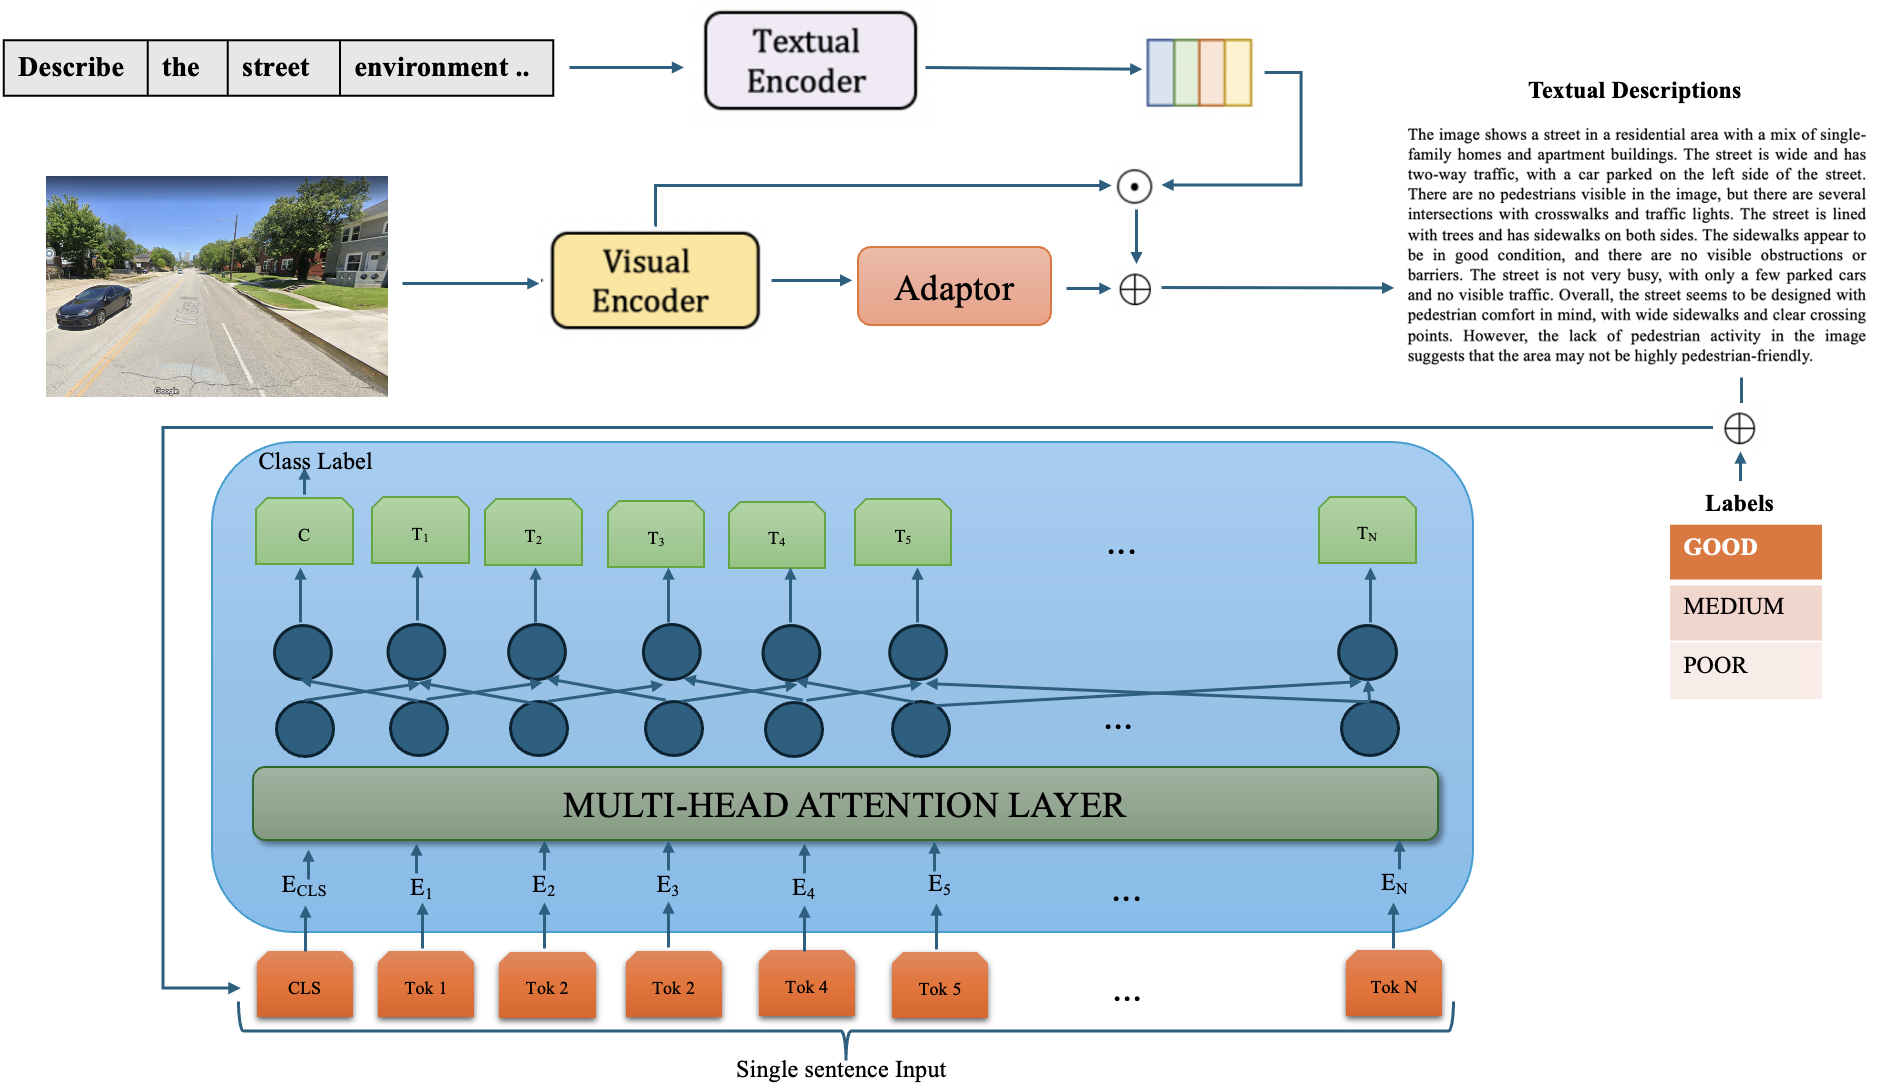
\includegraphics[width=0.9\linewidth]{image-Bert_classification.png}
    \caption{BERT classification with Vlm's Description}
    \label{fig:overview}
\end{figure}

At the core of BERT’s architecture lies its multi-layer transformer design, which relies on the scaled dot-product self-attention mechanism to capture relationships among tokens \citep{devlin2019bert}. This mechanism is defined as:
\begin{equation}
\text{Attention}(Q, K, V) = \mathrm{softmax}\!\biggl(\frac{Q K^T}{\sqrt{d_k}}\biggr) V,
\end{equation}
where \( Q \), \( K \), and \( V \) are the query, key, and value matrices derived from learned linear transformations of the input embeddings, and \( \sqrt{d_k} \) normalizes the dot product. Each transformer layer uses multi-head attention, enabling the model to learn diverse aspects of the sequence simultaneously. The outputs of these attention heads are concatenated and passed through a linear layer:
\begin{equation}
H = W_o \,\mathrm{concat}(\mathrm{head}_1, \mathrm{head}_2, \dots, \mathrm{head}_h),
\end{equation}
where \( W_o \) is a learned weight matrix. This refined representation is then sent to the final classification head.

To ensure the BERT classifier performed effectively, we trained it with a maximum token length of 128 and carefully tuned key hyperparameters—such as learning rate, batch size, and number of epochs. During fine-tuning, the model minimized the cross-entropy loss:
\begin{equation}
L = - \sum_{i=1}^{N} y_i \,\log P(y_i \mid x_i),
\end{equation}
where \( y_i \) is the ground-truth label for sample \( i \), and \( P(y_i \mid x_i) \) is the predicted probability of that label. This optimization process encouraged accurate predictions, and we evaluated the model’s success using classification accuracy, confirming the pipeline’s overall efficacy.

\subsection{VLM for Direct Classification}
In addition to applying VLMs for generating textual descriptions subsequently classified by BERT, we also explored the capability of VLMs for direct image classification. This approach bypasses the intermediate step of generating free-form text descriptions and instead utilizes the inherent multimodal understanding of the VLMs to directly predict the pedestrian-friendliness category of the input image.

For this direct classification task, we also employed the Molmo and Qwen-VL-Chat models. The input to these models consisted of the image itself, along with a structured query designed to elicit a classification response. For instance, a query could be phrased as "What is the pedestrian-friendliness level of this image? Answer with one of the following categories: [Category 1], [Category 2], [Category 3]." The specific categories would be replaced with the actual pedestrian-friendliness classes defined in our dataset. The VLMs, having been pre-trained on vast amounts of image-text data, possess an internal understanding of visual concepts and their semantic relationships. By providing the image and a constrained query specifying the desired output format (one of the predefined categories), we prompted the models to directly map the visual features of the image to the appropriate classification label \citep{bordes2024introduction}. The accuracy of this direct classification approach was then evaluated by comparing the VLM's predictions against the ground-truth labels in our dataset.

\section{Case Study}

\subsection{Data Collection}

In this study, we used an automated pipeline to collect Google Street View images from major cities around the world. The process was implemented in Python using the PyAutoGUI library \citep{sweigart2020pyautogui}. In total, approximately 10,000 images were collected from 16 different cities (Figure \ref{fig:all_cities}). And to avoid collecting duplicate images, we maintained a log of previously visited coordinates. Before capturing a new image, the script checks this log to ensure the selected coordinate hasn't been used before.

\begin{figure}[H]
    \centering
    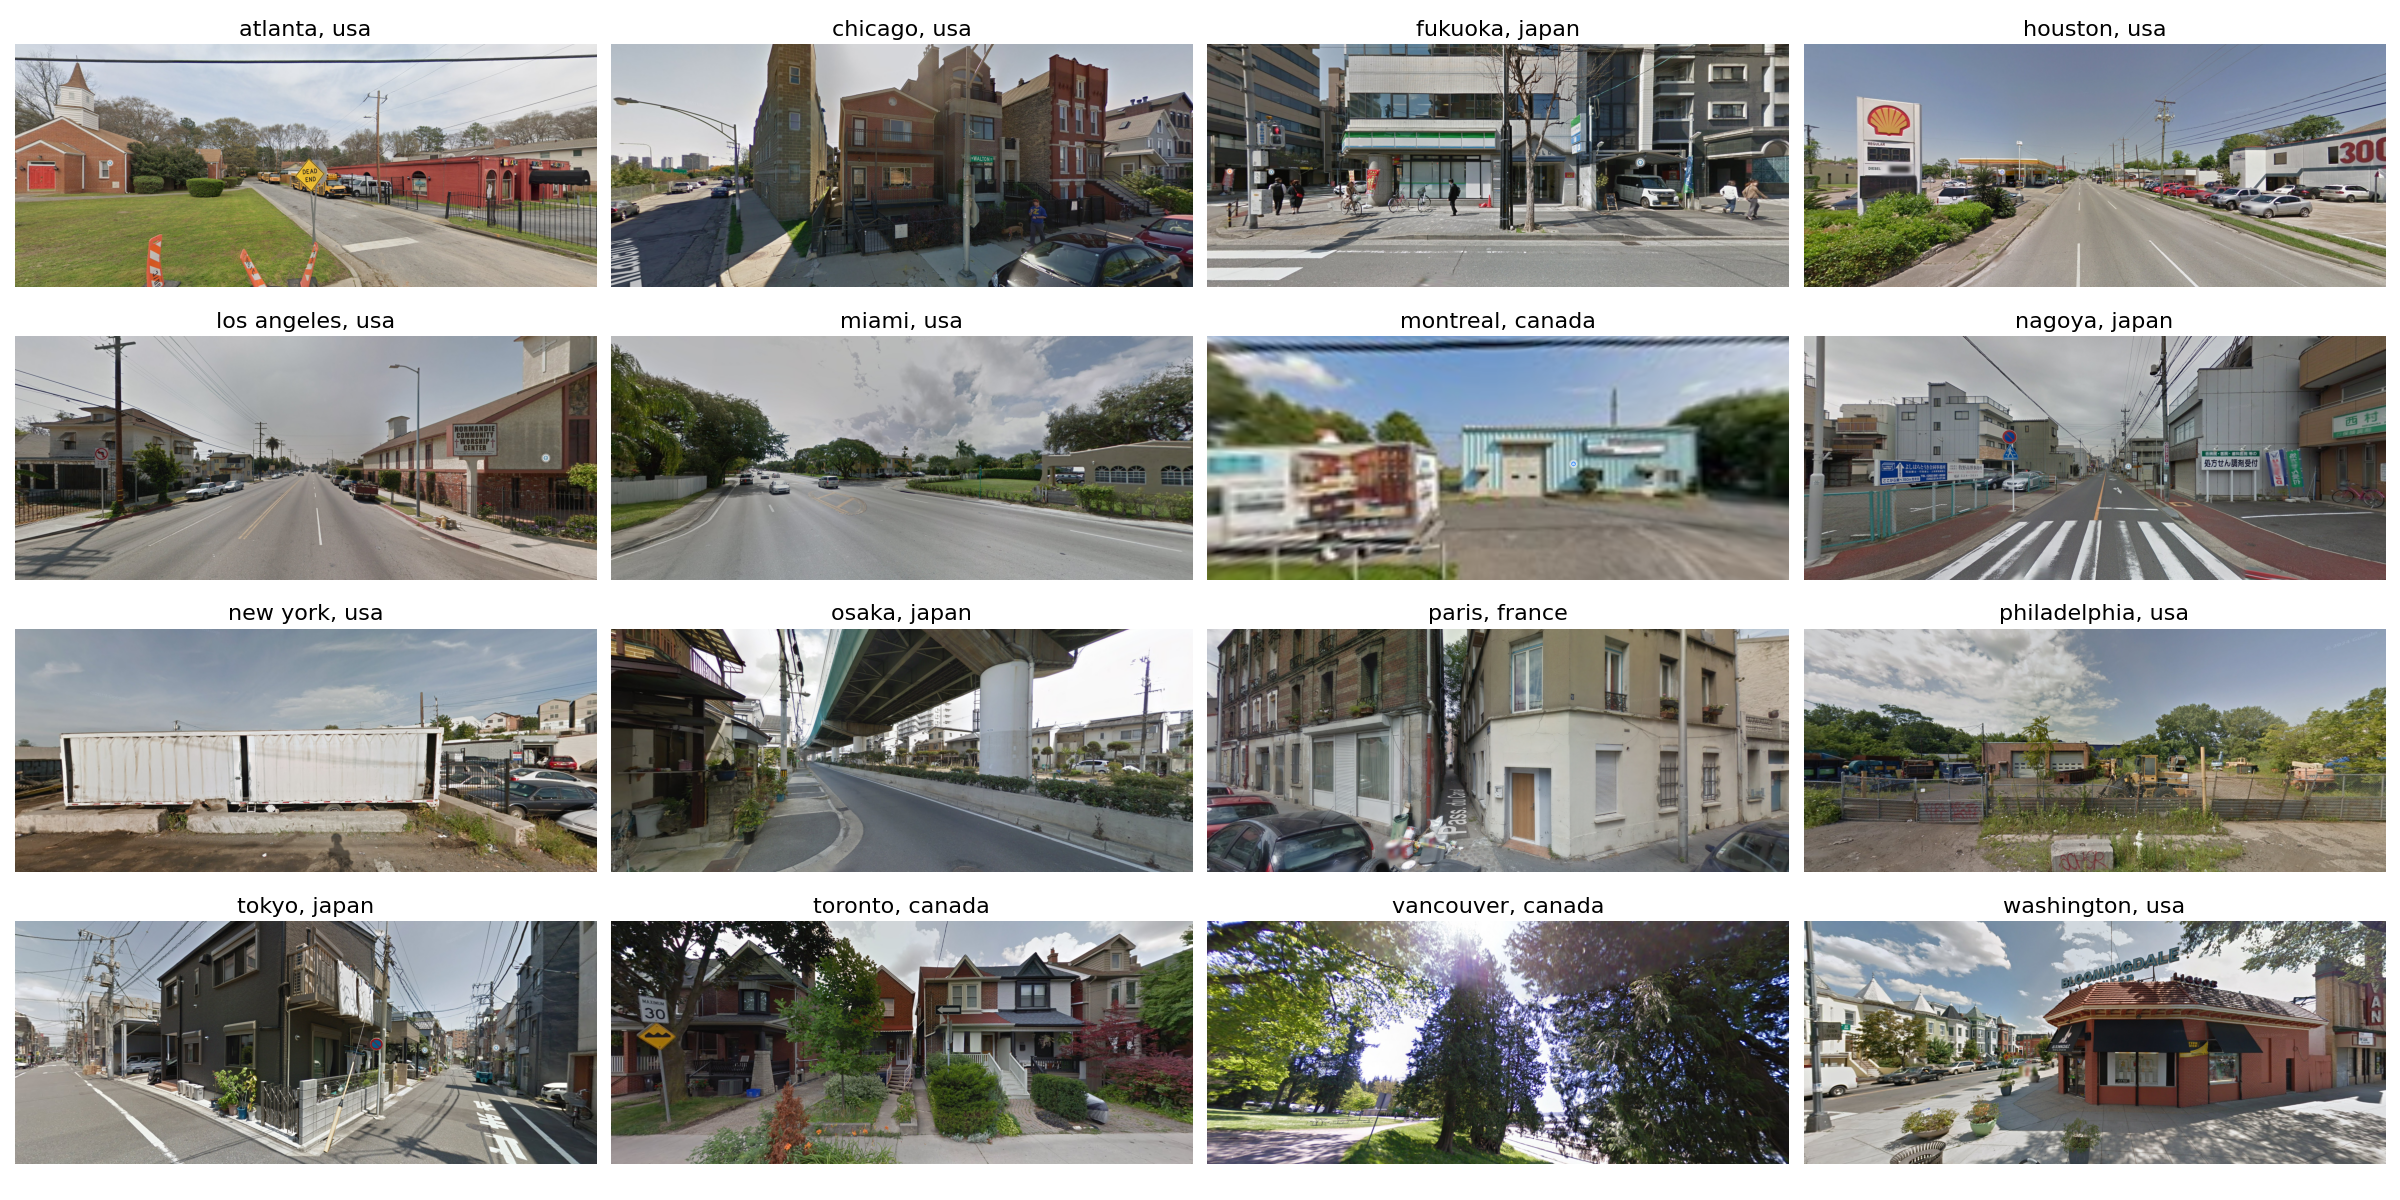
\includegraphics[width=0.9\linewidth]{all_cities.png}
    \caption{Sample Image Collected}
    \label{fig:all_cities}
\end{figure}

\subsection{Labeling Images with Average Rating }

After creating the image dataset, each image was evaluated based on six independent reviews. The final rating for each image is determined as the average of these six reviews. The ratings provided for the images are categorized into three levels:
\begin{itemize}
    \item Level 1: Poor – The area looks dull and uninviting. There are no natural features or interesting sights. It does not feel pleasant to walk there.
    \item Level 2: Moderate – The area has a mix of surroundings. There may be some natural features or points of interest, but not many. It’s an average place to walk.
    
    \item Level 3: Good – The area is attractive and enjoyable. It has lots of natural features and interesting things to see. It feels like a great place for walking.
\end{itemize}

Figure \ref{fig:rating} displays some sample images from the dataset, which provides a visual representation of the walking routes that have been evaluated and categorized according to the rating criteria mentioned above.


\begin{figure}[H]
    \centering
    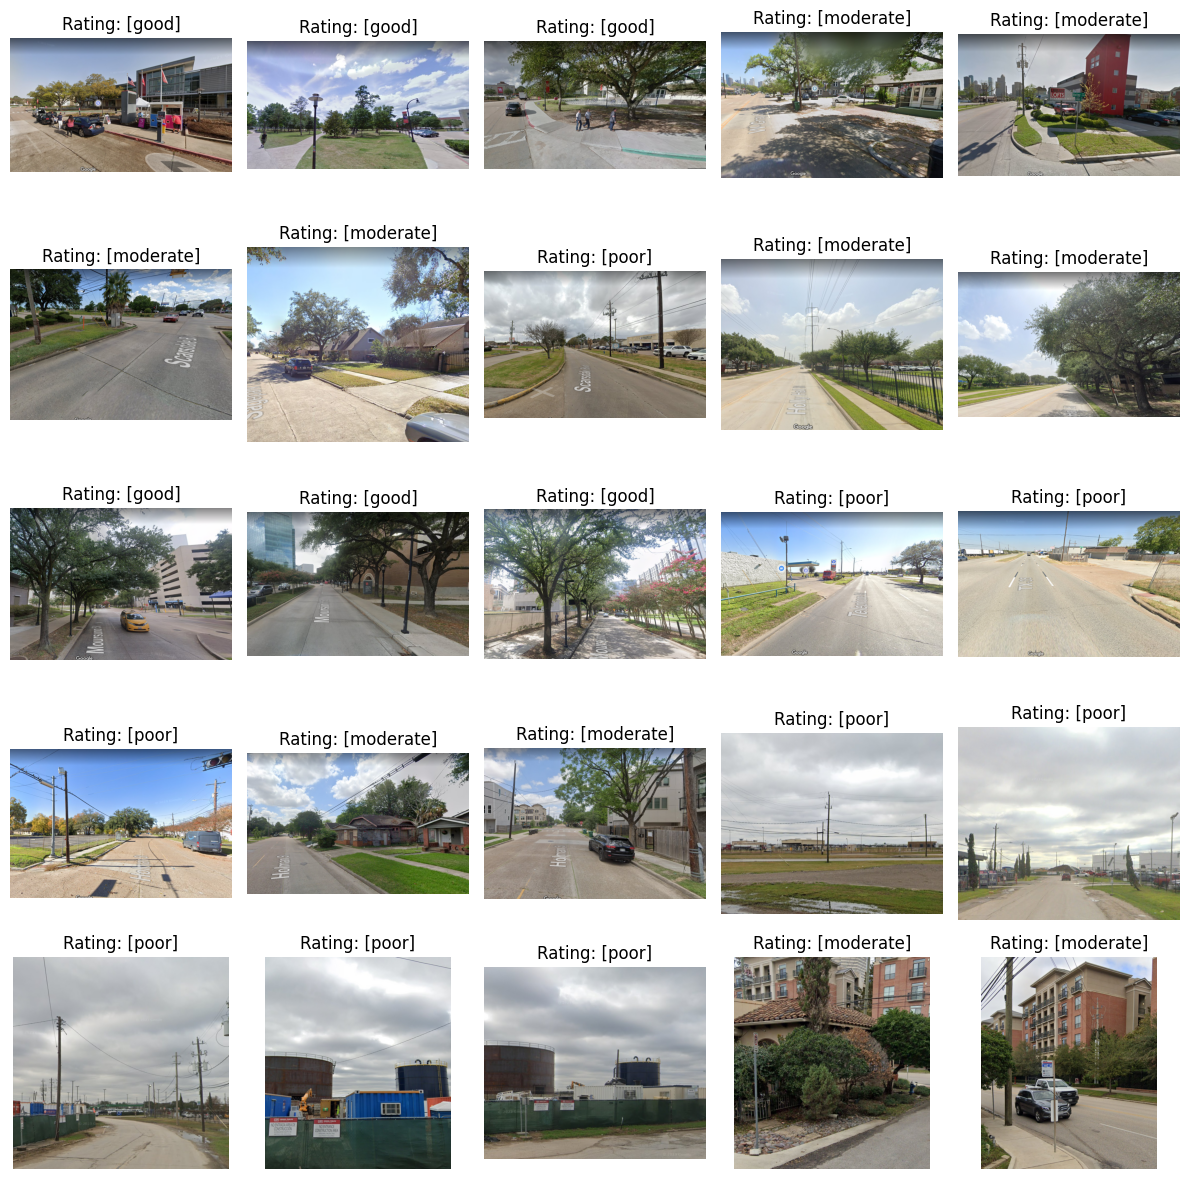
\includegraphics[width=0.7\linewidth]{rating.png}
    \caption{Sample Images and Ratings}
    \label{fig:rating}
\end{figure}



\subsection{Model Assessment}
In this research, we employed different metrics to evaluate the classification performance of the proposed model’s network. Accuracy assesses the model’s overall correctness, while precision focuses on the model's ability to accurately classify positive cases. Recall, on the other hand, evaluates the model’s capability to correctly identify negative samples. Additionally, the F1 score serves as a measure that balances precision and recall, providing a comprehensive evaluation of the classification performance.

\begin{equation}
    \text{Accuracy} = \frac{\text{correct classifications}}{\text{all classifications}}
\end{equation}

\begin{equation}
    \text{Precision} = \frac{TP}{TP + FP}
\end{equation}

\begin{equation}
    \text{Recall} = \frac{TP}{TP + FN}
\end{equation}

\begin{equation}
    F1 = \frac{2 \times \text{Recall} \times \text{Precision}}{\text{Recall} + \text{Precision}}
\end{equation}

In the context of classification evaluation, Equations (2)--(4) define key performance metrics. The term true positive (TP) represents instances where rating levels are correctly classified. Conversely, false positive (FP) denotes cases where rating levels are incorrectly classified. False negative (FN) represents rating levels that are correctly identified as non-members, while true negative (TN) represents non-members correctly identified.


\subsection{Results}

\subsubsection{CNN based Classification}
In this study, the model was built and trained using TensorFlow and Keras frameworks. The training process was consistent across all models, with 20 epochs and 0.001 learning rate as the optimized hyperparameters. Each training iteration handled a batch size of 32 samples. The performance comparison of the various models, including accuracy, macro average F1 score, and weighted average F1 score, is presented in Table \ref{tab:cnn_results}. The Macro Average F1 Score treats all classes equally, while the Weighted Average F1 Score considers class imbalances by giving more weight to larger classes. Notably, the ResNet50, InceptionV3, MobileNet, and MobileNetV2 outperformed other models, achieving accuracy levels of over 80\% in their predictions. Conversely, the EfficientNetB0 model displayed the lowest accuracies, only reaching 34\%.

% \hl{update this table}

\begin{table}[H]
    \centering
    \caption{Performance of Different Models on the Test Dataset}\label{tab:cnn_results}
    \begin{tabular}{l c c c}
        \toprule
        \textbf{Model} & \textbf{Accuracy} & \textbf{Macro Average F1 Score} & \textbf{Weighted Average F1 Score} \\
        \midrule
        MobileNet & 0.85 & 0.86 & 0.85 \\
        ResNet50 & 0.83 & 0.83 & 0.82 \\
        MobileNetV2 & 0.83 & 0.84 & 0.83 \\        
        InceptionV3 & 0.81 & 0.82 & 0.81 \\
        DenseNet121 & 0.75 & 0.75 & 0.73 \\
        InceptionResNetV2 & 0.67 & 0.67 & 0.66 \\
        VGG16 & 0.65 & 0.66 & 0.66 \\
        VGG19 & 0.56 & 0.56 & 0.55 \\        
        EfficientNetB0 & 0.34 & 0.17 & 0.17 \\
        \bottomrule
    \end{tabular}
\end{table}

Figure~\ref{fig:curves} presents the training and validation loss curves for all the models we fine-tuned. These plots help assess how well each model generalizes and whether they are prone to overfitting or underfitting. All models demonstrate a clear downward trend in training loss, indicating effective learning from the training data. MobileNet and MobileNet V2 maintain a close alignment between training and validation losses throughout the epochs, which suggests that there is a good generalization and minimal overfitting. VGG16 and VGG19 show relatively stable loss curves, although occasional fluctuations in validation loss may indicate mild overfitting. Moreover, ResNet50 and DenseNet121 exhibit more noticeable gaps between training and validation losses, especially in the later epochs, which indicates a higher risk of overfitting after certain epochs. Inception V3 and InceptionResNetV2 show generally decreasing trends in both losses but experience some volatility in the validation loss, especially in the mid to later epochs. EfficientNet B0 appears to converge quickly within a few epochs, though its validation loss fluctuates, possibly due to the small number of training epochs. Overall, while all models improve over time, lightweight architectures such as MobileNet variants tend to provide more stable and consistent generalization, whereas deeper models like ResNet50 and InceptionResNetV2 may require more careful tuning to avoid overfitting.

% \hl{use pdf, seaborn format}

\begin{figure}[H]
    \centering
    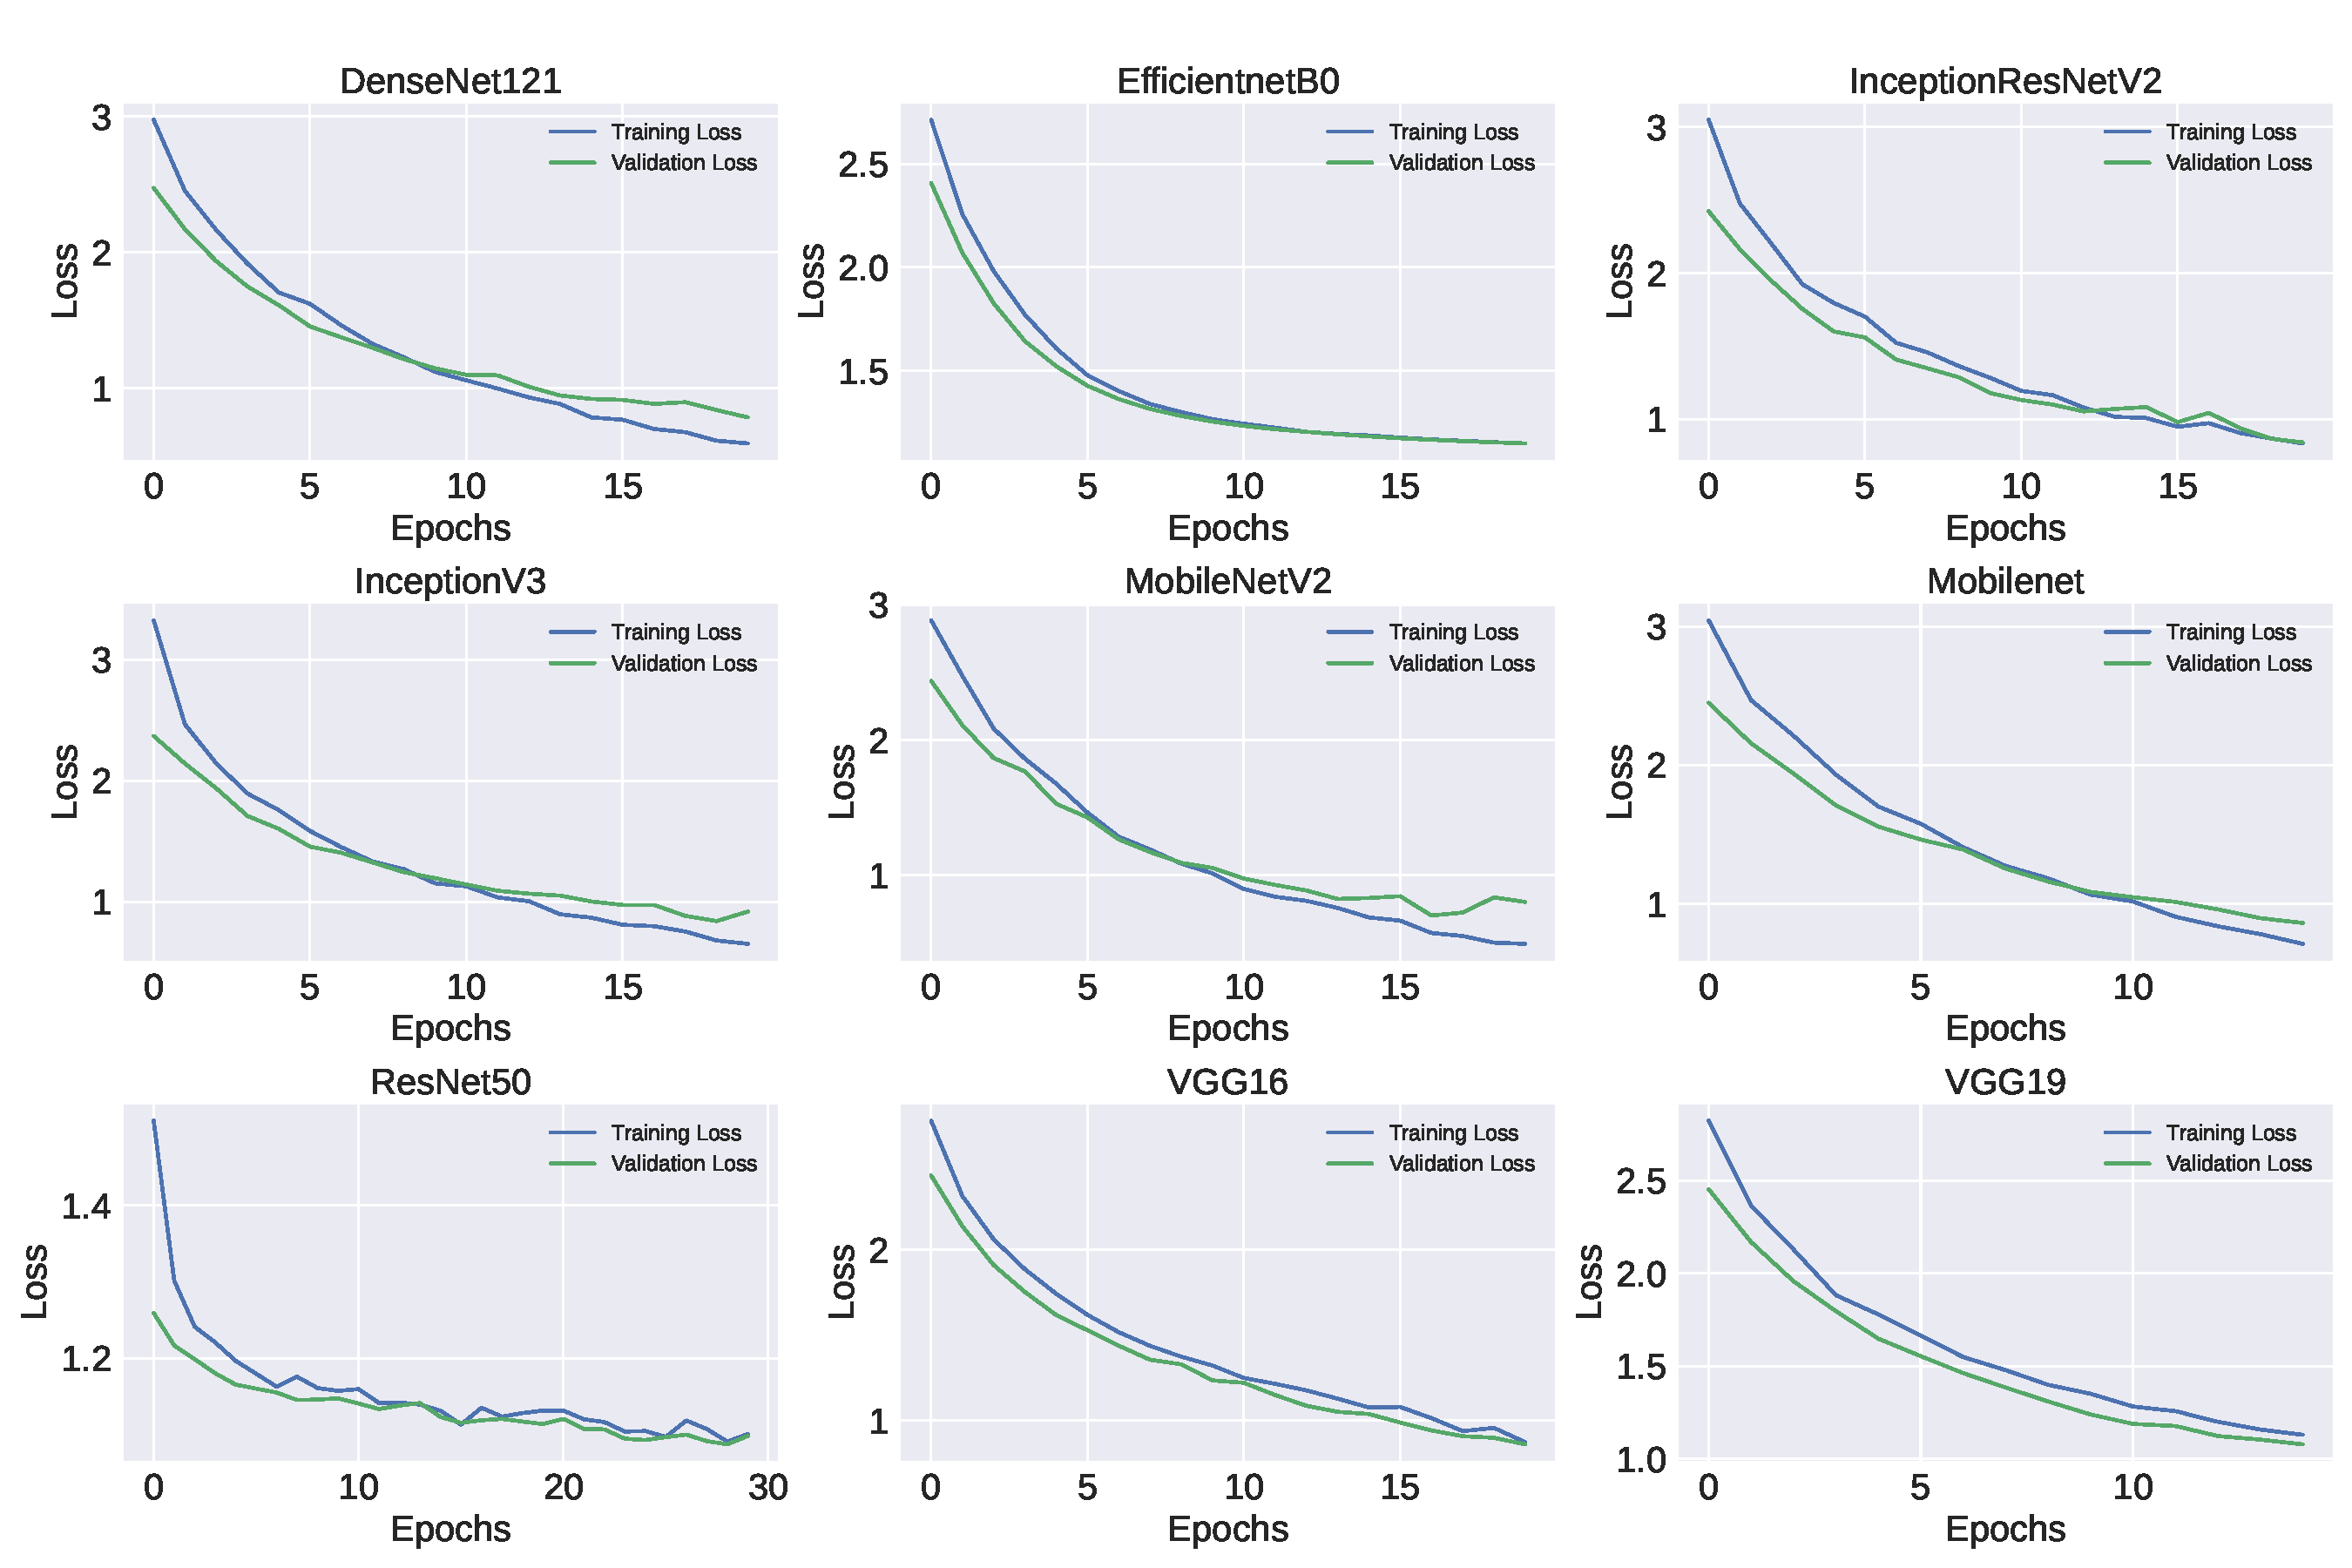
\includegraphics[width=1.0\linewidth]{all_models_loss_curves_new_font.pdf}
    \caption{Loss Curves for all CNN Models}
    \label{fig:curves}
\end{figure}

After evaluating individual model performance, we selected ResNet50, InceptionV3, MobileNet, and MobileNetV2 as the top-performing models to include in an ensemble. The ensemble was built using a weighted voting strategy, where each model, trained independently, cast a vote for the predicted class, and the final prediction was determined by the class receiving the highest total weight.

The performance of the ensemble model is summarized in Table~\ref{tab:ensemble}, which reports classification metrics across the three classes: Good, Moderate, and Poor. The model achieved high precision, recall, and F1 scores for all classes, indicating well-balanced and reliable performance. Specifically, the F1 score for both the ‘Good’ and ‘Poor’ classes reached 0.909, while the ‘Moderate’ class had a slightly lower F1 score of 0.875. These results reflect strong agreement between predicted and actual labels, particularly for the ‘Good’ class, which had the highest recall at 0.972. Overall, the ensemble model achieved class-level accuracies of 0.951, 0.903, and 0.938 for Good, Moderate, and Poor categories, respectively. The macro average and weighted average F1 scores were 0.89 and 0.90, which confirms the ensemble’s effectiveness in leveraging the strengths of multiple models to enhance classification accuracy.

\begin{table}[H]
\centering
\caption{Per-Class Classification Metrics for ensemble model}
\label{tab:ensemble}
\begin{tabular}{lccccc}
\hline
\textbf{Class} & \textbf{Precision} & \textbf{Recall} & \textbf{F1 Score} & \textbf{Accuracy} \\
\hline
Good     & 0.854 & 0.972 & 0.909 & 0.951 \\
Moderate & 0.925 & 0.831 & 0.875 & 0.903 \\
Poor     & 0.900 & 0.918 & 0.909 & 0.938 \\
\hline
\end{tabular}
\end{table}


\subsubsection{Vision Language Model with BERT classification}
In this approach, we use VML to generate a text description, which is then used to train a classification model. Below is an example VLM prompt used to generate text description: \newline

\textbf{Prompt:} \textit{Describe the street environment in the image in as much detail as possible, focusing on elements relevant to pedestrian-friendliness and walkability analysis. Identify key features such as buildings, roads, intersections, sidewalks, crosswalks, pedestrian pathways, public spaces, and the presence of pedestrians. Assess the availability, width, and condition of sidewalks, as well as any barriers or obstructions that may affect pedestrian movement. Describe the relationship between vehicles and pedestrians, including traffic density, crossing points, and potential pedestrian safety concerns. Mention the presence of public amenities such as benches, bus stops, shaded areas, and accessibility features. Provide a structured and thorough analysis of the scene from the perspective of pedestrian comfort, safety, and accessibility for urban walkability evaluation.}   \newline


Figure~\ref{fig:enter-label_molmo_description} displays the text descriptions generated by the Molmo model, which takes both an image and a text prompt as inputs. Rather than presenting a single block of text, Molmo structures its output into clear points that analyze the street environment. Notably, it provides detailed observations about key elements such as buildings, roads, and overall neighborhood layout.

\begin{figure}[H]
    \centering
    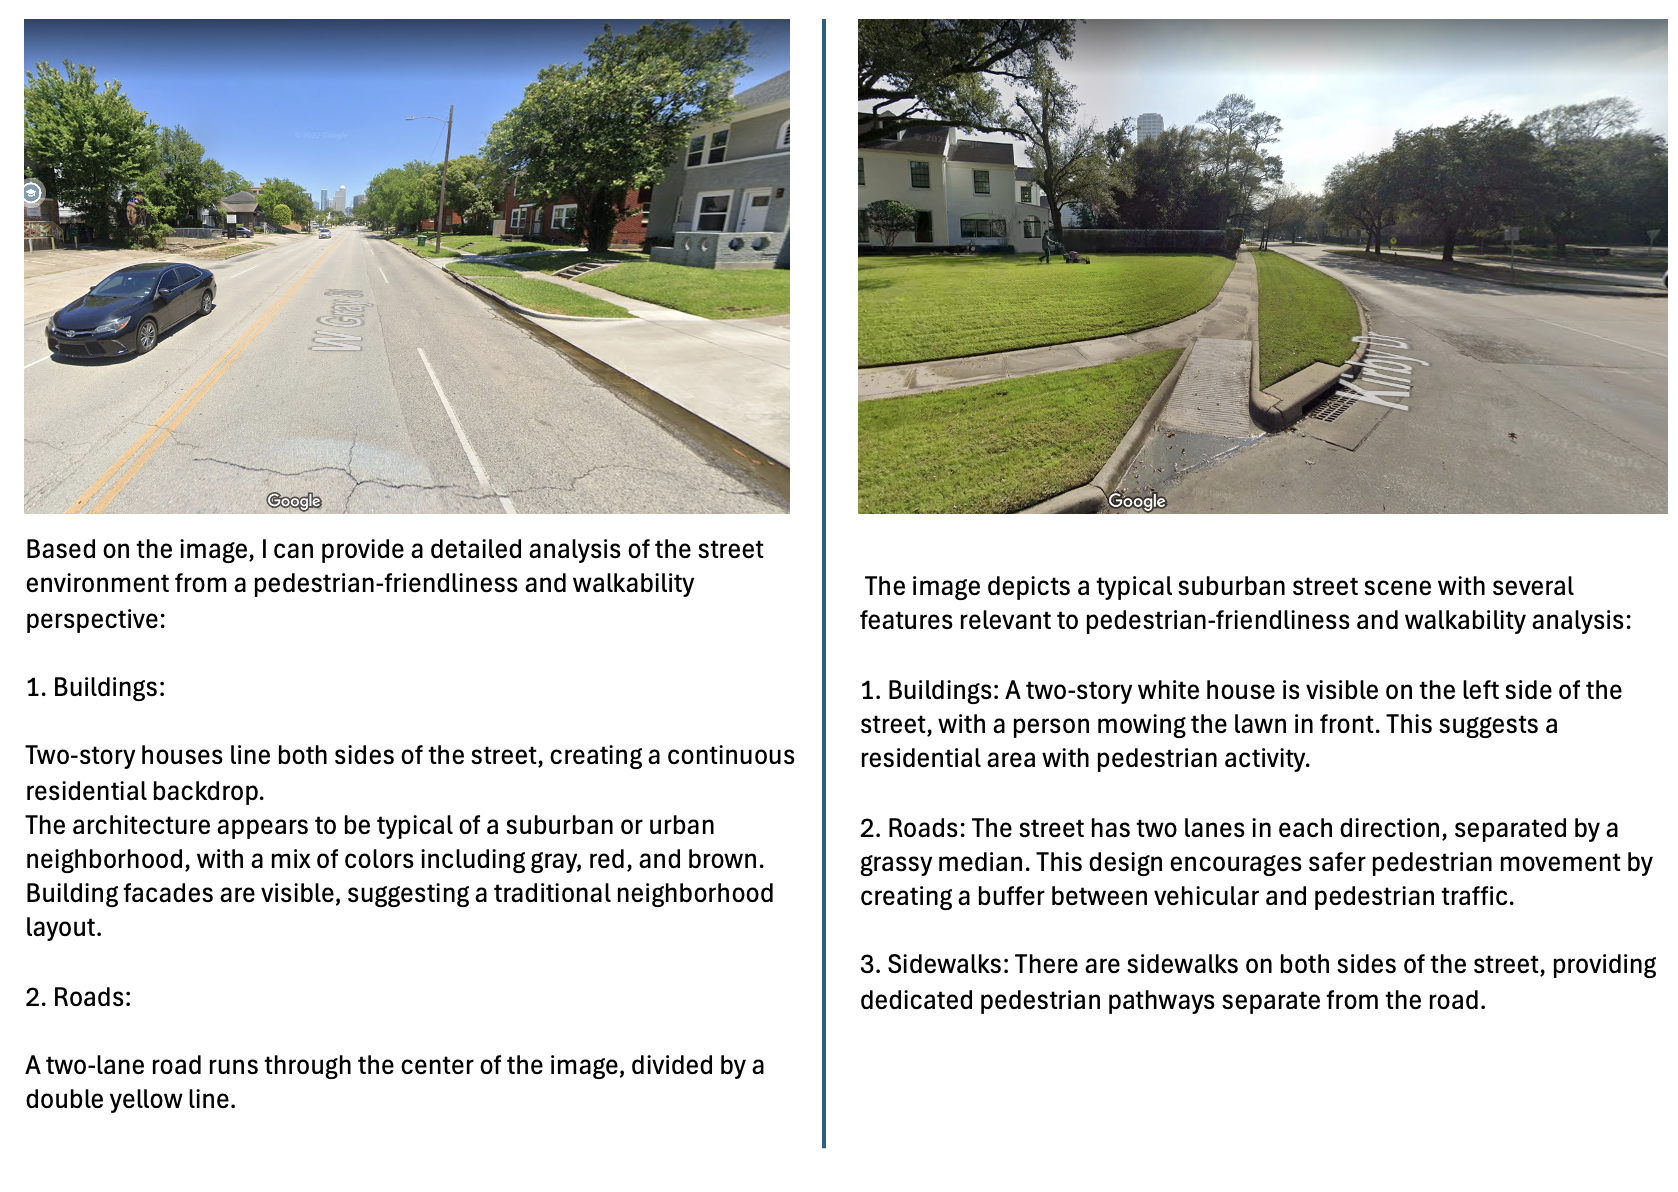
\includegraphics[width=1.0\linewidth]{image_molmo_descriptions.png}
    \caption{Molmo Generated descriptions}
    \label{fig:enter-label_molmo_description}
\end{figure}

Figure~\ref{fig:enter-label_qwen_description} shows the text descriptions generated by Qwen-VL-Chat. It focuses on key pedestrian-friendliness factors, such as the presence of sidewalks, traffic lights, and neighborhood conditions. After generating the text descriptions, ratings were assigned to each one based on the ground-truth labels from the original dataset. The dataset was then split, with 80\% used for training and 20\% reserved for final testing. Within the training portion, we further partitioned the data: using 80\% for actual training and 20\% for validation. The validation set was used for hyperparameter tuning. We tokenized the text data using the fast BERT tokenizer, which sets a maximum sequence length of 128 tokens and applies both padding and truncation to ensure consistent input formatting. The classification head of the pre-trained BERT base model was modified to predict three classes: good, moderate, and poor. To balance performance and efficiency, we froze the first nine layers of the model, which allows only the top three layers to be fine-tuned. 

\begin{figure}[H]
    \centering
    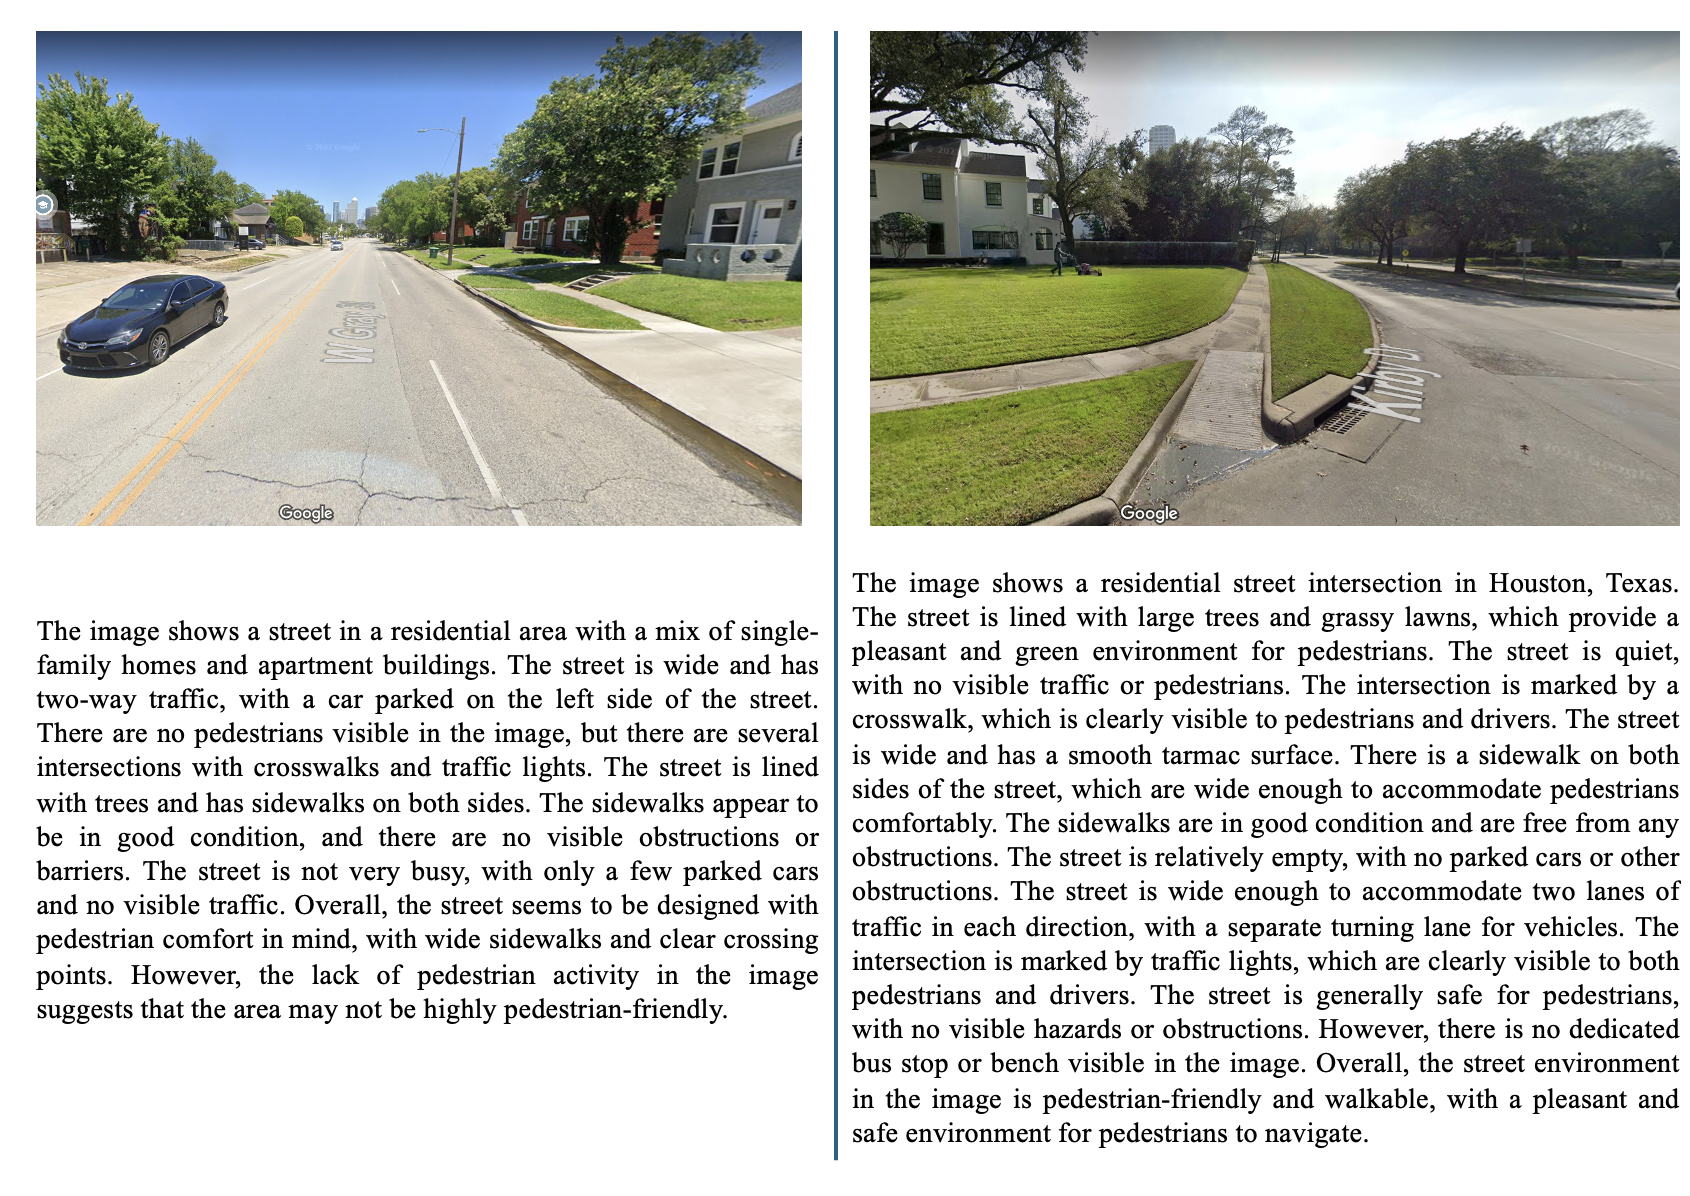
\includegraphics[width=1.0\linewidth]{image_qwen_descriptions.png}
    \caption{Qwen-VL-Chat descriptions}
    \label{fig:enter-label_qwen_description}
\end{figure}



Figure~\ref{fig:vlm_curves} presents the training and validation loss curves for BERT models trained using text descriptions generated by Qwen-VL-Chat (left) and Molmo (right). The Qwen-VL-Chat model shows a steady and consistent decline in both training and validation loss across epochs, which indicates stable convergence and effective learning. Notably, the validation loss follows the training loss closely, with no significant divergence, which suggests the model generalizes well without overfitting. In contrast, the Molmo-trained model exhibits a more modest decrease in training loss and a slightly erratic pattern in validation loss. The validation loss initially rises, suggesting possible overfitting, but then drops and aligns with the training loss by the third epoch. This fluctuation suggests that while the Molmo model eventually starts to learn meaningful patterns, its training stability and generalization performance are less consistent compared to the Qwen-VL-Chat model. Overall, the Qwen-VL-Chat–based training demonstrates more robust and reliable learning behavior. 



% \hl{pdf}


\begin{figure}[H]
  \centering
  \begin{subfigure}[b]{0.45\textwidth}
    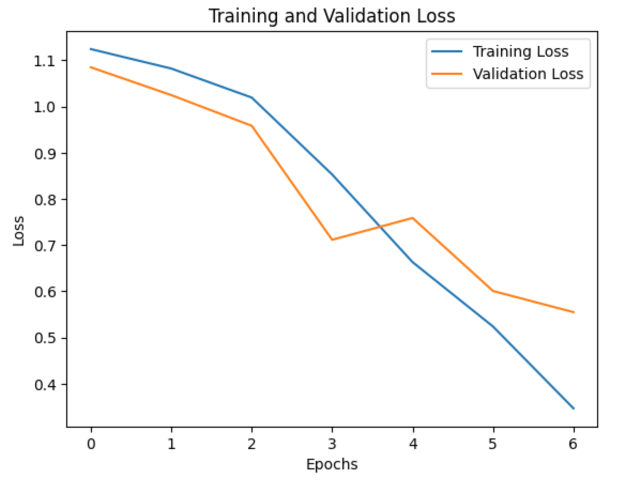
\includegraphics[width=\textwidth]{image_bert_results.png}
    \caption{Qwen-VL-Chat}
  \end{subfigure}
  \hspace{0.05\textwidth}
  \begin{subfigure}[b]{0.45\textwidth}
    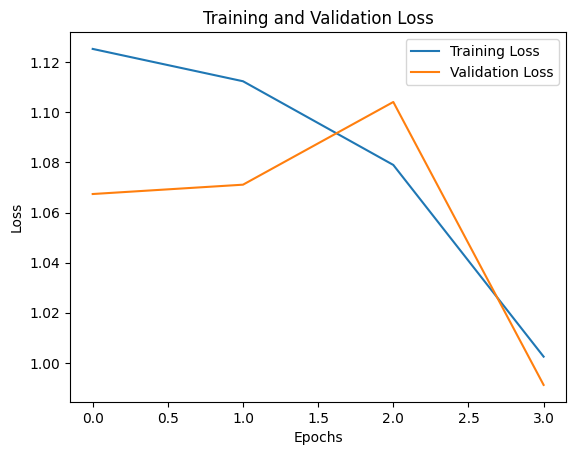
\includegraphics[width=\textwidth]{image_molmo_loss.png}
    \caption{Molmo}
  \end{subfigure}
  \caption{Loss Curves for VLM-BERT Models}
  \label{fig:vlm_curves}
\end{figure}




Table~\ref{tab:bert_table} presents the classification results comparing BERT models trained on Qwen-VL-chat and Molmo-generated descriptions. The Qwen-VL-chat model performs well across all three classes with balanced precision, recall, and F1-scores. It achieves high precision for the Poor class (0.9189), reducing false positives, while its recall (0.6415) indicates some missed instances. For the Moderate class, strong recall (0.8125) suggests effective identification of true cases. The Good class shows both high precision (0.8000)and recall ({0.9302}), resulting in a strong F1-score of {0.8602}. The Molmo-based BERT model shows weaker performance overall. For the Poor class, it achieves lower precision (0.7222), a low recall (0.3939), and a modest F1-score of 0.5098. In the Moderate class, performance improves, with recall (0.7500), moderate precision (0.5538), and an F1-score of (0.6371). However, for the Good class, the model's both precision (0.5294) and recall (0.4737) are low. Overall, the Qwen-VL-chat model demonstrates consistently strong and balanced performance across all categories, while the Molmo model shows instability and lower effectiveness, particularly in correctly identifying Poor and Good instances. 

% \hl{four 0.9000}


\begin{table}[H]
\centering
\caption{Comparison of BERT Classification Results: Qwen-VL-chat vs. Molmo}
\label{tab:bert_table}
\begin{tabular}{l|cccc|cccc}
\hline
\multirow{2}{*}{\textbf{Class}} & \multicolumn{4}{c|}{\textbf{Qwen-VL-chat}} & \multicolumn{4}{c}{\textbf{Molmo}} \\
 & \textbf{Precision} & \textbf{Recall} & \textbf{F1-score} & \textbf{Accuracy} & \textbf{Precision} & \textbf{Recall} & \textbf{F1-score} & \textbf{Accuracy} \\
\hline
Poor     & 0.9189 & 0.6415 & 0.7556 & 0.6415 & 0.7222 & 0.3939 & 0.5098 & 0.3939 \\
Moderate & 0.6842 & 0.8125& 0.7429 & 0.8125 & 0.5538 & 0.7500 & 0.6371 & 0.7500 \\
Good     & 0.8000 & 0.9302 & 0.8602 & 0.9104 & 0.5294 & 0.4737 & 0.5000 & 0.4737 \\
\hline
\end{tabular}
\end{table}


\subsubsection{Direct Vision Language Model classification}

We also tested using VLM to directly classify images into these three classes: Good, Moderate, and Poor. Figure~\ref{fig:direct} shows sample images classified by Molmo and Qwen-VL-Chat direclty with a predefined prompt (as shown below), along with their corresponding comparisons to human-assigned ratings. 


\begin{quote}
\textbf{Prompt:} \textit{You are an expert in urban design and pedestrian safety. Analyze the Google Street View image and assess whether the environment shown is suitable for pedestrians. Consider features such as the presence and condition of sidewalks, pedestrian crossings, traffic levels, shade, lighting, and the separation between pedestrians and vehicles. Also take into account the general cleanliness, accessibility, and the presence of amenities like benches, signage, or storefronts that support walking. Based on your analysis, classify the pedestrian environment as Good, Moderate, or Poor. Then provide a brief explanation (2–3 sentences) justifying your rating by referencing specific visual features from the image.}
\end{quote}

\begin{figure}[H]
    \centering
    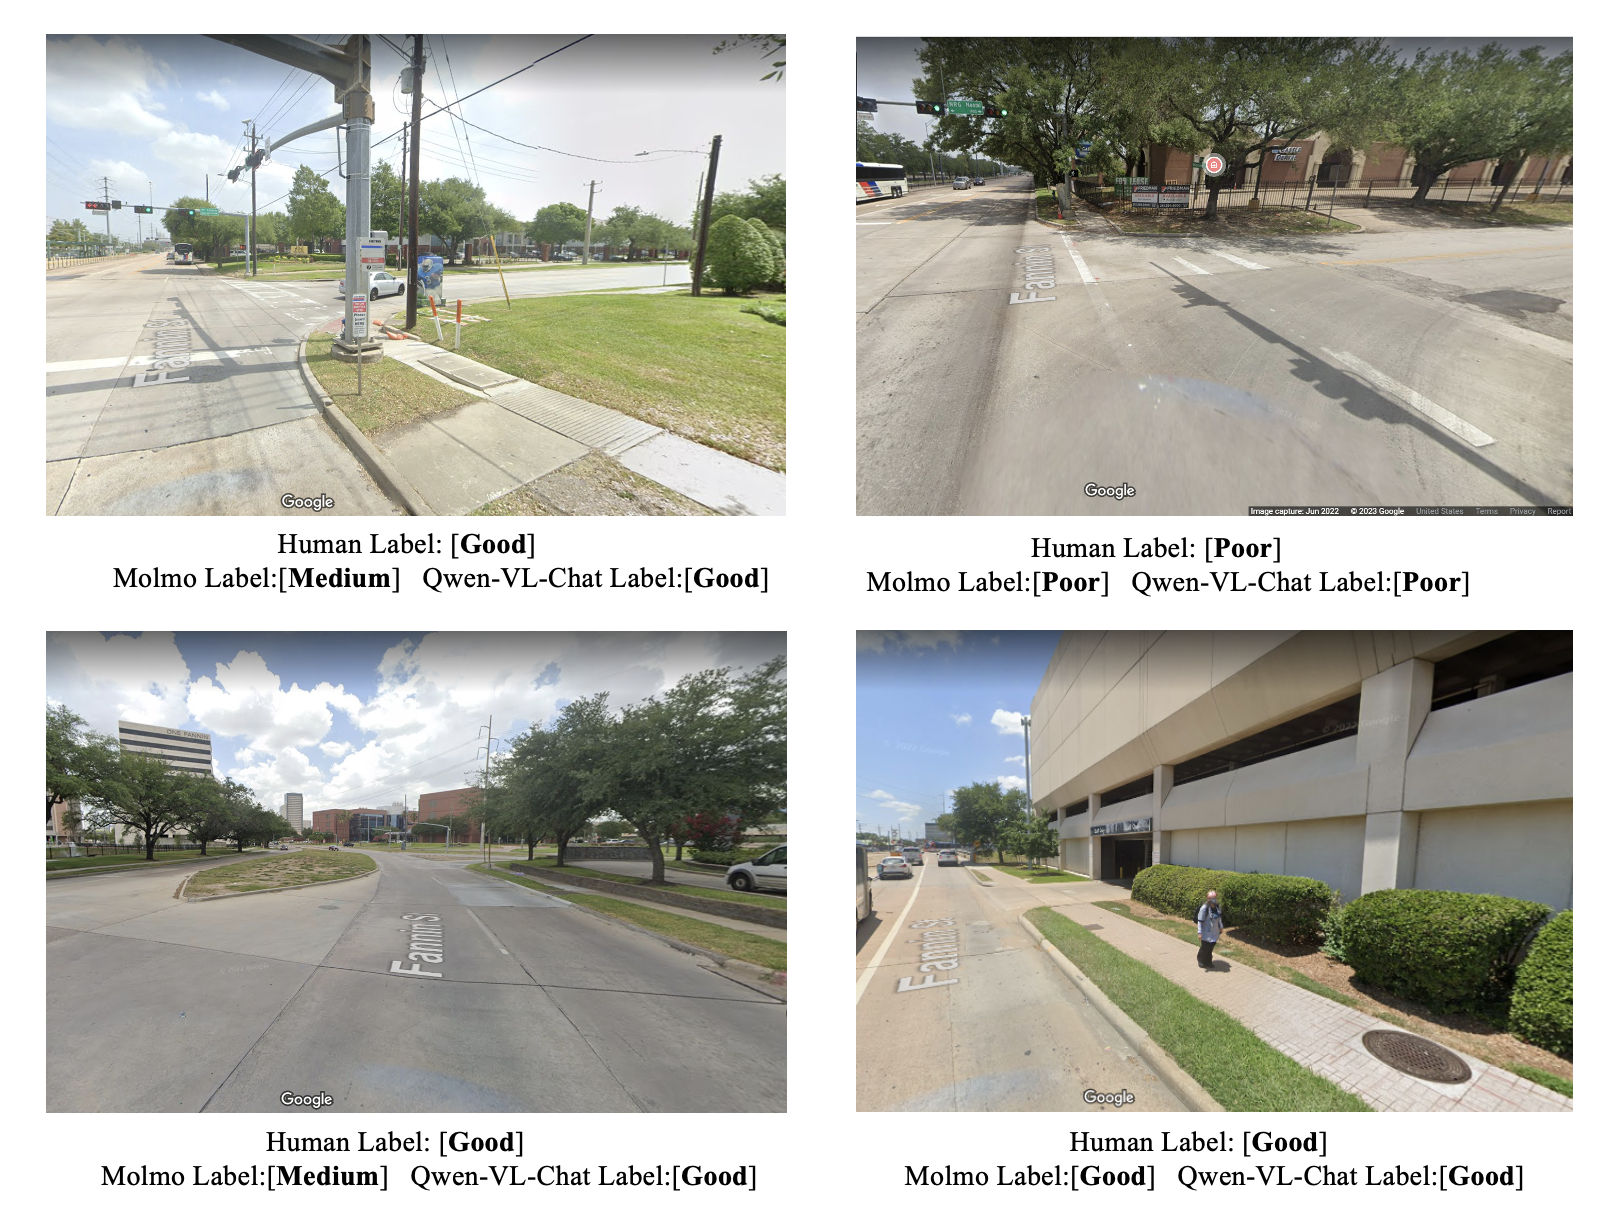
\includegraphics[width=0.8\linewidth]{image_direct_qwen.png}
    \caption{Images with Human Labels with Molmo,Qwen Generated Labels }
    \label{fig:direct}
\end{figure}


Table~\ref{tab:direct_compare} presents the classification performance of the Qwen-VL-Chat and Molmo models across the good, moderate, and poor labels. For the good class, Qwen-VL-Chat achieves a high recall of 0.77 but low precision (0.27), indicating it identifies most good samples but with many false positives. Molmo shows even lower precision (0.13) but still maintains a relatively high recall (0.65), resulting in a higher F1-score (0.60) than Qwen-VL-Chat (0.40). For the moderate class, Qwen-VL-Chat demonstrates a more balanced performance with precision and recall around 0.40, which leads to an F1-score of 0.41. Molmo, while achieving the same precision (0.43), has a lower recall (0.25), resulting in a notably lower F1-score of 0.17. In the poor class, Qwen-VL-Chat achieves perfect precision (1.00) but an extremely low recall (0.02), indicating it predicts the poor label with high certainty but fails to capture almost all actual poor cases. Molmo, on the other hand, provides a more modest precision (0.82) and slightly better recall (0.13), leading to a higher F1-score (0.16) compared to Qwen-VL-Chat’s 0.05. Overall, Qwen-VL-Chat tends to favor precision, particularly for the poor class, at the cost of recall, while Molmo delivers slightly more balanced but still limited performance across all classes. These results indicate that direct classification using VLM is less effective than approaches that leverage VLM generated descriptions combined with BERT. The latter method consistently produces more accurate and reliable classifications. 

\begin{table}[H]
\centering
\caption{Comparison of Direct Classification Reports: Qwen-VL-Chat vs. Molmo}
\label{tab:direct_compare}
\begin{tabular}{l|cccc|cccc}
\hline
\multirow{2}{*}{\textbf{Label}} & \multicolumn{4}{c|}{\textbf{Qwen-VL-Chat}} & \multicolumn{4}{c}{\textbf{Molmo}} \\
 & \textbf{Precision} & \textbf{Recall} & \textbf{F1-Score} & \textbf{Support} & \textbf{Precision} & \textbf{Recall} & \textbf{F1-Score} & \textbf{Support} \\
\hline
Good      & 0.27 & 0.77 & 0.40 & 94  & 0.13 & 0.65 & 0.60 & 94  \\
Moderate  & 0.43 & 0.40 & 0.41 & 240 & 0.43 & 0.25 & 0.17 & 240 \\
Poor      & 1.00 & 0.02 & 0.05 & 163 & 0.82 & 0.13 & 0.16 & 163 \\
\hline
\end{tabular}
\end{table}

\subsection{Discussions}
The performance of different architectures in classifying pedestrian-friendliness of street environments reveals several important insights. First, the CNN-based classification experiments underscore the effectiveness of fine-tuning well-known architectures. Several models exhibited relatively high accuracy (above 80\%). The subsequent ensemble of the top-four CNN models further improved performanceto around 90\% accuracy. 

In the VLM-BERT approach, the text descriptions generated by Qwen-VL-Chat produced more coherent and detailed cues for pedestrian-friendliness, which has balanced precision, recall, and F1-scores across the three classes (good, moderate, and poor). In contrast, the descriptions provided by Molmo, while still capturing some street-level features, exhibited more variability and led to lower classification metrics. This discrepancy suggests that the quality and specificity of VLM-generated text directly impact downstream classification tasks. Moreover, fine-tuning BERT on the textual data proved more effective than directly prompting VLMs for classification. While prompting Molmo and Qwen-VL-Chat to directly label the images did yield some correct predictions, the overall metrics were notably weaker than those achieved through the two-stage pipeline (text generation followed by BERT classification). This finding reinforces the importance of specialized training and indicates that current VLMs may still benefit from synergy with task-specific models in more complex or domain-sensitive scenarios.

\section{CONCLUSIONS}
This study introduced a suite of deep learning–based methods to automatically evaluate pedestrian friendliness in urban streetscapes using Google Street View images. By using CNN architectures and VLMs, our experiments demonstrated how machine learning can capture visual cues related to walkability and correlate them with human-rated comfort, safety, and accessibility.

We explored three distinct approaches. First, using transfer learning on pre-trained CNN architectures like ResNet50, MobileNet, and InceptionV3, we achieved high classification accuracy. An ensemble of the top-performing models further improved results, which reaches nearly 90\% accuracy. Second, a two-stage pipeline that generated textual descriptions using VLMs followed by classification with a fine-tuned BERT model also performed strongly, especially when using Qwen-VL-Chat, with accuracy around 85\% and well-balanced F1-scores across all classes. Finally, we tested a direct classification approach using VLMs alone, which produced lower and more unstable performance. 

Despite these promising outcomes, several limitations remain. Pedestrian-friendliness labels, based on six raters’ opinions, still carry subjectivity and potential bias. Also, using only static images limits our ability to account for dynamic factors like time of day, weather, or temporary obstructions. Moreover, the models focused only on visual inputs, overlooking influential non-visual data such as traffic volume, crime statistics, or proximity to amenities. Future research should aim to expand the dataset across more cities, seasons, and environments to improve generalizability. Gathering input from a more diverse group of annotators can help reduce bias in labeling. Integrating other types of urban data such as infrastructure quality, real-time traffic conditions, or safety reports would enrich model predictions. Further work could also explore explainability and fine-tuning for VLMs, or deploy active learning to continually refine predictions using human-in-the-loop feedback. 




% \section*{Declarations}


% \subsection*{Funding}
% This research received no external funding.
% \subsection*{Conflict of interest}
% The authors declare no conflict of interest.
% \subsection*{Ethics approval and consent to participate}
% Not applicable.
% \subsection*{Consent for publication}
% Not applicable.
% \subsection*{Data availability}
% The datasets generated during the current study are available from the corresponding author on reasonable request.
% \subsection*{Author contribution}

% Prathyush Kumar Reddy Lebaku conducted the data analysis and contributed to the drafting of the manuscript. Dr. Lu Gao supervised the research, developed the study design, and finalized the manuscript. Dr. Kailai Wang provided guidance on methodology and assisted with result interpretation. Dr. Jingran Sun contributed to the literature review and provided critical revisions. All authors read and approved the final manuscript.

%Bibliography
\bibliographystyle{unsrtnat}
\bibliography{references}  



\end{document}
